\documentclass[a4paper,fleqn]{cas-dc}

\usepackage[numbers]{natbib}
\usepackage{graphicx}
\usepackage{xcolor}
\usepackage{listings}
\usepackage{float}
\usepackage{caption}
\usepackage{booktabs}
\usepackage{subcaption}
\usepackage{hyperref}
\usepackage{cuted}

\usepackage{amsthm}
\newtheorem*{note}{Note}

\definecolor{codegreen}{rgb}{0,0.6,0}
\definecolor{codegray}{rgb}{0.5,0.5,0.5}
\definecolor{backcolour}{rgb}{0.97,0.97,0.97} 

\lstdefinestyle{mystyle}{
	backgroundcolor=\color{backcolour},   
	commentstyle=\color{codegreen}\itshape, 
	keywordstyle=\color{blue}\bfseries,     
	numberstyle=\tiny\color{codegray},      
	basicstyle=\ttfamily\footnotesize,     
	breakatwhitespace=false,         
	breaklines=true,                
	captionpos=b,                    
	keepspaces=true,                 
	numbers=none,                   
	showspaces=false,                
	showstringspaces=false,
	showtabs=false,                  
	tabsize=4,                      
	frame=single,                    
	rulecolor=\color{lightgray}      
}

\lstset{style=mystyle, 
	aboveskip=10pt,  
	belowskip=10pt   
}

\def\tsc#1{\csdef{#1}{\textsc{\lowercase{#1}}\xspace}}
\tsc{WGM}
\tsc{QE}
\tsc{EP}
\tsc{PMS}
\tsc{BEC}
\tsc{DE}
%%%
\makeatletter
\def\printorcid{}
\makeatother

\begin{document}
\let\WriteBookmarks\relax
\def\floatpagepagefraction{1}
\def\textpagefraction{.001}


\shorttitle{A Neuro-Symbolic Architecture for Pneumonia Detection} 
\shortauthors{N. Flego et al.} 

% --- Titolo Principale ---
\title[mode = title]{A Neuro-Symbolic Hybrid Architecture for Robust Pneumonia Detection and Localization in Chest X-rays} 

% =======================================================
% --- Autore 1 (Primo Autore e Corresponding Author) ---
% =======================================================
\author[1,2]{Nicola Flego}
\cormark[1] % Indica che sei il corresponding author
\ead{n1flego@edu.aau.at} % Corretto il refuso n1flego
\credit{Conceptualization, Software Development, Data Analysis, Writing - Original Draft}

% =======================================================
% --- Autore 2 ---
% =======================================================
\author[1,2]{Filippo Pilutti} % Il [1,2] indica che appartiene a entrambe le affiliazioni (rimuovi il 2 se non serve)
\ead{filippopi@edu.aau.at}
\credit{Conceptualization, Software Development, Data Analysis}

% =======================================================
% --- Autore 3 ---
% =======================================================
\author[1]{Mohamed El Bahnasawi}
\ead{mohamed.elbahnasawi@aau.at}
\credit{Supervision}

% =======================================================
% --- Autore 4 ---
% =======================================================
\author[1]{Kyandoghere Kyamakya}
\ead{kyandoghere.kyamakya@aau.at}
\credit{Supervision}

% =======================================================
% --- Affiliazioni ---
% =======================================================

% Affiliazione 1 (Principale)
\affiliation[1]{organization={University of Klagenfurt (AAU)},
	addressline={Universitätsstraße 65-67}, 
	city={Klagenfurt am Wörthersee},
	postcode={9020}, 
	country={Austria}}

% Affiliazione 2 (Da usare se un coautore è di un'altra università/ospedale)
\affiliation[2]{organization={Università degli Studi di Udine (UNIUD)},
	addressline={Via Palladio, 8}, 
	city={Udine},
	postcode={33100}, 
	country={Italy}}

% --- Note a piè di pagina ---
\cortext[cor1]{Corresponding author}

% --- Abstract ---
\begin{abstract}
Visual localization and robust image recognition in unstructured or medical environments remain significant challenges due to the performance degradation of standard Convolutional Neural Networks (CNNs) under noise, low lighting, or artifacts. This report proposes a novel hybrid neuro-symbolic architecture designed to enhance the reliability of pneumonia detection and localization in Chest X-rays (CXRs).

The system integrates a Cellular Neural Network (CeNN) frontend, which leverages continuous-time dynamics to provide intrinsic noise-suppression and edge preservation, with a DenseNet-121 backbone optimized via domain-specific transfer learning. To bridge the gap between statistical perception and anatomical reasoning, the pipeline incorporates a Semantic Validation Module based on Answer Set Programming (ASP). This logic-based layer acts as a post-inference gate, evaluating neural predictions against a Knowledge Base of geometric and biological constraints to filter "hallucinations" and rescue sub-threshold clinical cases.

Experimental results on the RSNA Pneumonia dataset demonstrate that the CeNN frontend maintains stable feature extraction even under 90\% Gaussian noise, where standalone CNNs structurally collapse. Furthermore, the neuro-symbolic integration significantly improves clinical safety, reducing False Negatives, outperforming the best purely statistical thresholding approach. Despite the additional logical overhead, the system maintains high operational efficiency with a total inference time of 82 ms per image on consumer-grade hardware. This work establishes a path toward more transparent, safety-first AI tools for critical clinical triage.
\end{abstract}

% --- Keywords ---
\begin{keywords}
	Neuro-symbolic AI \sep Cellular Neural Networks \sep Pneumonia Detection \sep Answer Set Programming \sep Noise Robustness \sep Medical Image Localization
\end{keywords}

\maketitle

\section{Introduction}

Visual localization and robust image recognition in unstructured environments remain significant challenges in modern computer vision. While Convolutional Neural Networks (CNNs) have achieved state-of-the-art performance in ideal conditions, their accuracy often degrades significantly when input images are corrupted by noise, low lighting, or sensor artifacts. In real-world clinical scenarios, ensuring the reliability of the feature extraction process is critical for maintaining high diagnostic accuracy and precise anatomical localization.

To address these limitations, this project proposes a hybrid neural architecture that leverages the intrinsic properties of Cellular Neural Networks (CeNN). Unlike traditional fully connected networks, CeNNs constitute a paradigm of information processing based on local interactions between cells. This architecture is particularly advantageous for image pre-processing and feature extraction, as its coupled dynamics allow for efficient noise filtering and edge preservation before the data is passed to higher-level classification layers.

The core of the proposed system is the integration of a CeNN-based front-end with a high-dimensional descriptor. Specifically, the network is designed to map visual inputs into a 512-dimensional feature space. This high-dimensional embedding allows the system to generate a unique "fingerprint" for each location or object, maintaining distinctiveness even when the original signal is heavily distorted by Gaussian or impulsive noise.

To further enhance the capabilities of the hybrid network, following the initial image classification and bounding box localization, all neural predictions are forwarded to an Answer Set Programming (ASP) module for semantic refinement. This critical step improves overall reliability by filtering out potential visual hallucinations and rescuing sub-threshold predictions where the neural network lacked sufficient confidence, thereby confirming the presence of pathology in borderline cases.

This report details the implementation, training, and evaluation of this hybrid approach. 

All experiments were conducted using a custom Python framework, analyzing the trade-off between computational complexity and recognition accuracy.

\section{Background}

Modern image recognition and localization systems rely heavily on Convolutional Neural Networks (CNNs). While these networks are effective when analyzing clear, high-quality images, their performance tends to degrade significantly in real-world environments due to factors like low light, sensor noise, or transmission errors. To address this limitation, this project utilizes Cellular Neural Networks (CeNN), a computing paradigm inspired by biological systems where each processing unit is connected only to its immediate neighbors. This local connectivity mimics the behavior of the human retina, allowing the network to process information based on local interactions rather than analyzing the global context immediately. Consequently, CeNNs are exceptionally capable at low-level image processing tasks, such as filtering random noise, enhancing edges, and filling in missing parts of an image. The core motivation of this work is to combine this intrinsic robustness with the classification power of modern feature extractors. We propose a hybrid system where a CeNN layer acts as a front-end pre-processor to stabilize and clean the input signal before it is mapped into a 512-dimensional feature space. This approach aims to bridge the gap between raw image processing and high-level semantic understanding, ensuring correct localization even when the input quality is compromised.

\subsection{Related Work}
The development of robust and interpretable diagnostic systems intersects multiple research domains, primarily standard Deep Learning for medical imaging, Cellular Neural Networks (CeNNs) for noise mitigation, and Neuro-Symbolic Artificial Intelligence.

\textbf{Deep Learning in Medical Imaging.} Standard Convolutional Neural Networks (CNNs) have achieved remarkable results in detecting pathologies from Chest X-rays (CXRs), including the RSNA Pneumonia dataset. Architectures such as ResNet and DenseNet \cite{densenet} are routinely employed as feature extractors due to their hierarchical representation capabilities. However, empirical studies demonstrate that purely statistical models are highly susceptible to out-of-distribution data, such as sensor noise, motion blur, or low-quality acquisitions common in resource-constrained environments. Furthermore, CNNs act as statistical "black boxes", lacking mechanisms to guarantee the anatomical plausibility of their predictions, which frequently leads to high-confidence false positives (hallucinations).

\textbf{CeNNs and Fault-Tolerant Architectures.} To address the fragility of standard CNNs, Cellular Neural Networks (CeNNs) \cite{CeNN} offer a paradigm based on local connectivity and continuous-time dynamics. Traditionally used in analog hardware for edge-preserving filtering and real-time image processing, CeNNs possess intrinsic noise-suppression capabilities. Recent conceptual frameworks, such as the edge-ready architecture proposed by Kutabuna et al. \cite{kubakisa20XXnoisy}, have highlighted the potential of integrating CeNN-inspired modules as robust frontends in medical pipelines. By stabilizing the input signal before deep feature extraction, CeNNs prevent the propagation of artifacts into the higher semantic layers. Our project directly draws inspiration from this paradigm, implementing a discrete-time CeNN layer to shield the DenseNet backbone from extreme Gaussian noise.

\textbf{Neuro-Symbolic AI and Semantic Validation.} The integration of explicit medical knowledge into deep learning pipelines is an emerging frontier designed to restore clinical trust. Neuro-symbolic systems aim to combine the perceptual strength of neural networks with the strict rule-enforcement of symbolic logic. While traditional models rely entirely on global statistical thresholds, semantic validation modules utilizing logic programming, such as Answer Set Programming (ASP) \cite{asp}, allow for the encoding of spatial and anatomical constraints (e.g., the position of the cardiac silhouette or the organic shape of a lung opacity). As suggested by the overarching architecture in \cite{kubakisa20XXnoisy}, employing logic to act as a post-inference gate enables the system to filter out geometrically impossible predictions. Our work operationalizes this concept, demonstrating the quantitative superiority of neuro-symbolic triage over standard statistical thresholding on a large-scale dataset.

\section{Dataset and Pre-processing}
\label{sec:dataset}

\subsection{Dataset Description}
The model was developed and evaluated using the dataset from the \textit{RSNA Pneumonia Detection Challenge}~\cite{rsna-pneumonia-detection-challenge}, hosted on Kaggle. This dataset is a subset of the NIH ChestX-ray14\cite{NIH-chest-xray} database and consists of anonymized chest radiographs (CXRs) in DICOM format. The dataset includes both normal cases and cases exhibiting lung opacities (pneumonia), alongside other abnormal conditions.

For the supervision of the learning process, the provided \texttt{stage\_2\_train\_labels.csv} file was used. This file contains ground truth information, including the binary classification target (0 for normal/no opacity, 1 for lung opacity) and the bounding box coordinates $(x, y, width, height)$ for the localization task.

\subsection{Data Partitioning and Balancing}
The original training set was split into training and validation subsets with a ratio of 80:20, using a fixed random seed for reproducibility. 

To address the class imbalance inherent in the dataset (there's a prevalence of normal/no-opacity cases compared to positive pneumonia cases), a weighted sampling strategy was implemented. A \texttt{WeightedRandomSampler} was applied to the training DataLoader, assigning a weight $w_i$ to each sample inversely proportional to the class frequency:
\begin{equation}
	w_c = \frac{1}{N_c}
\end{equation}
where $N_c$ is the number of samples for class $c$. This ensures that the model sees a balanced distribution of positive and negative cases during each training epoch.
	
\noindent
\begin{minipage}{\linewidth}
	\centering
	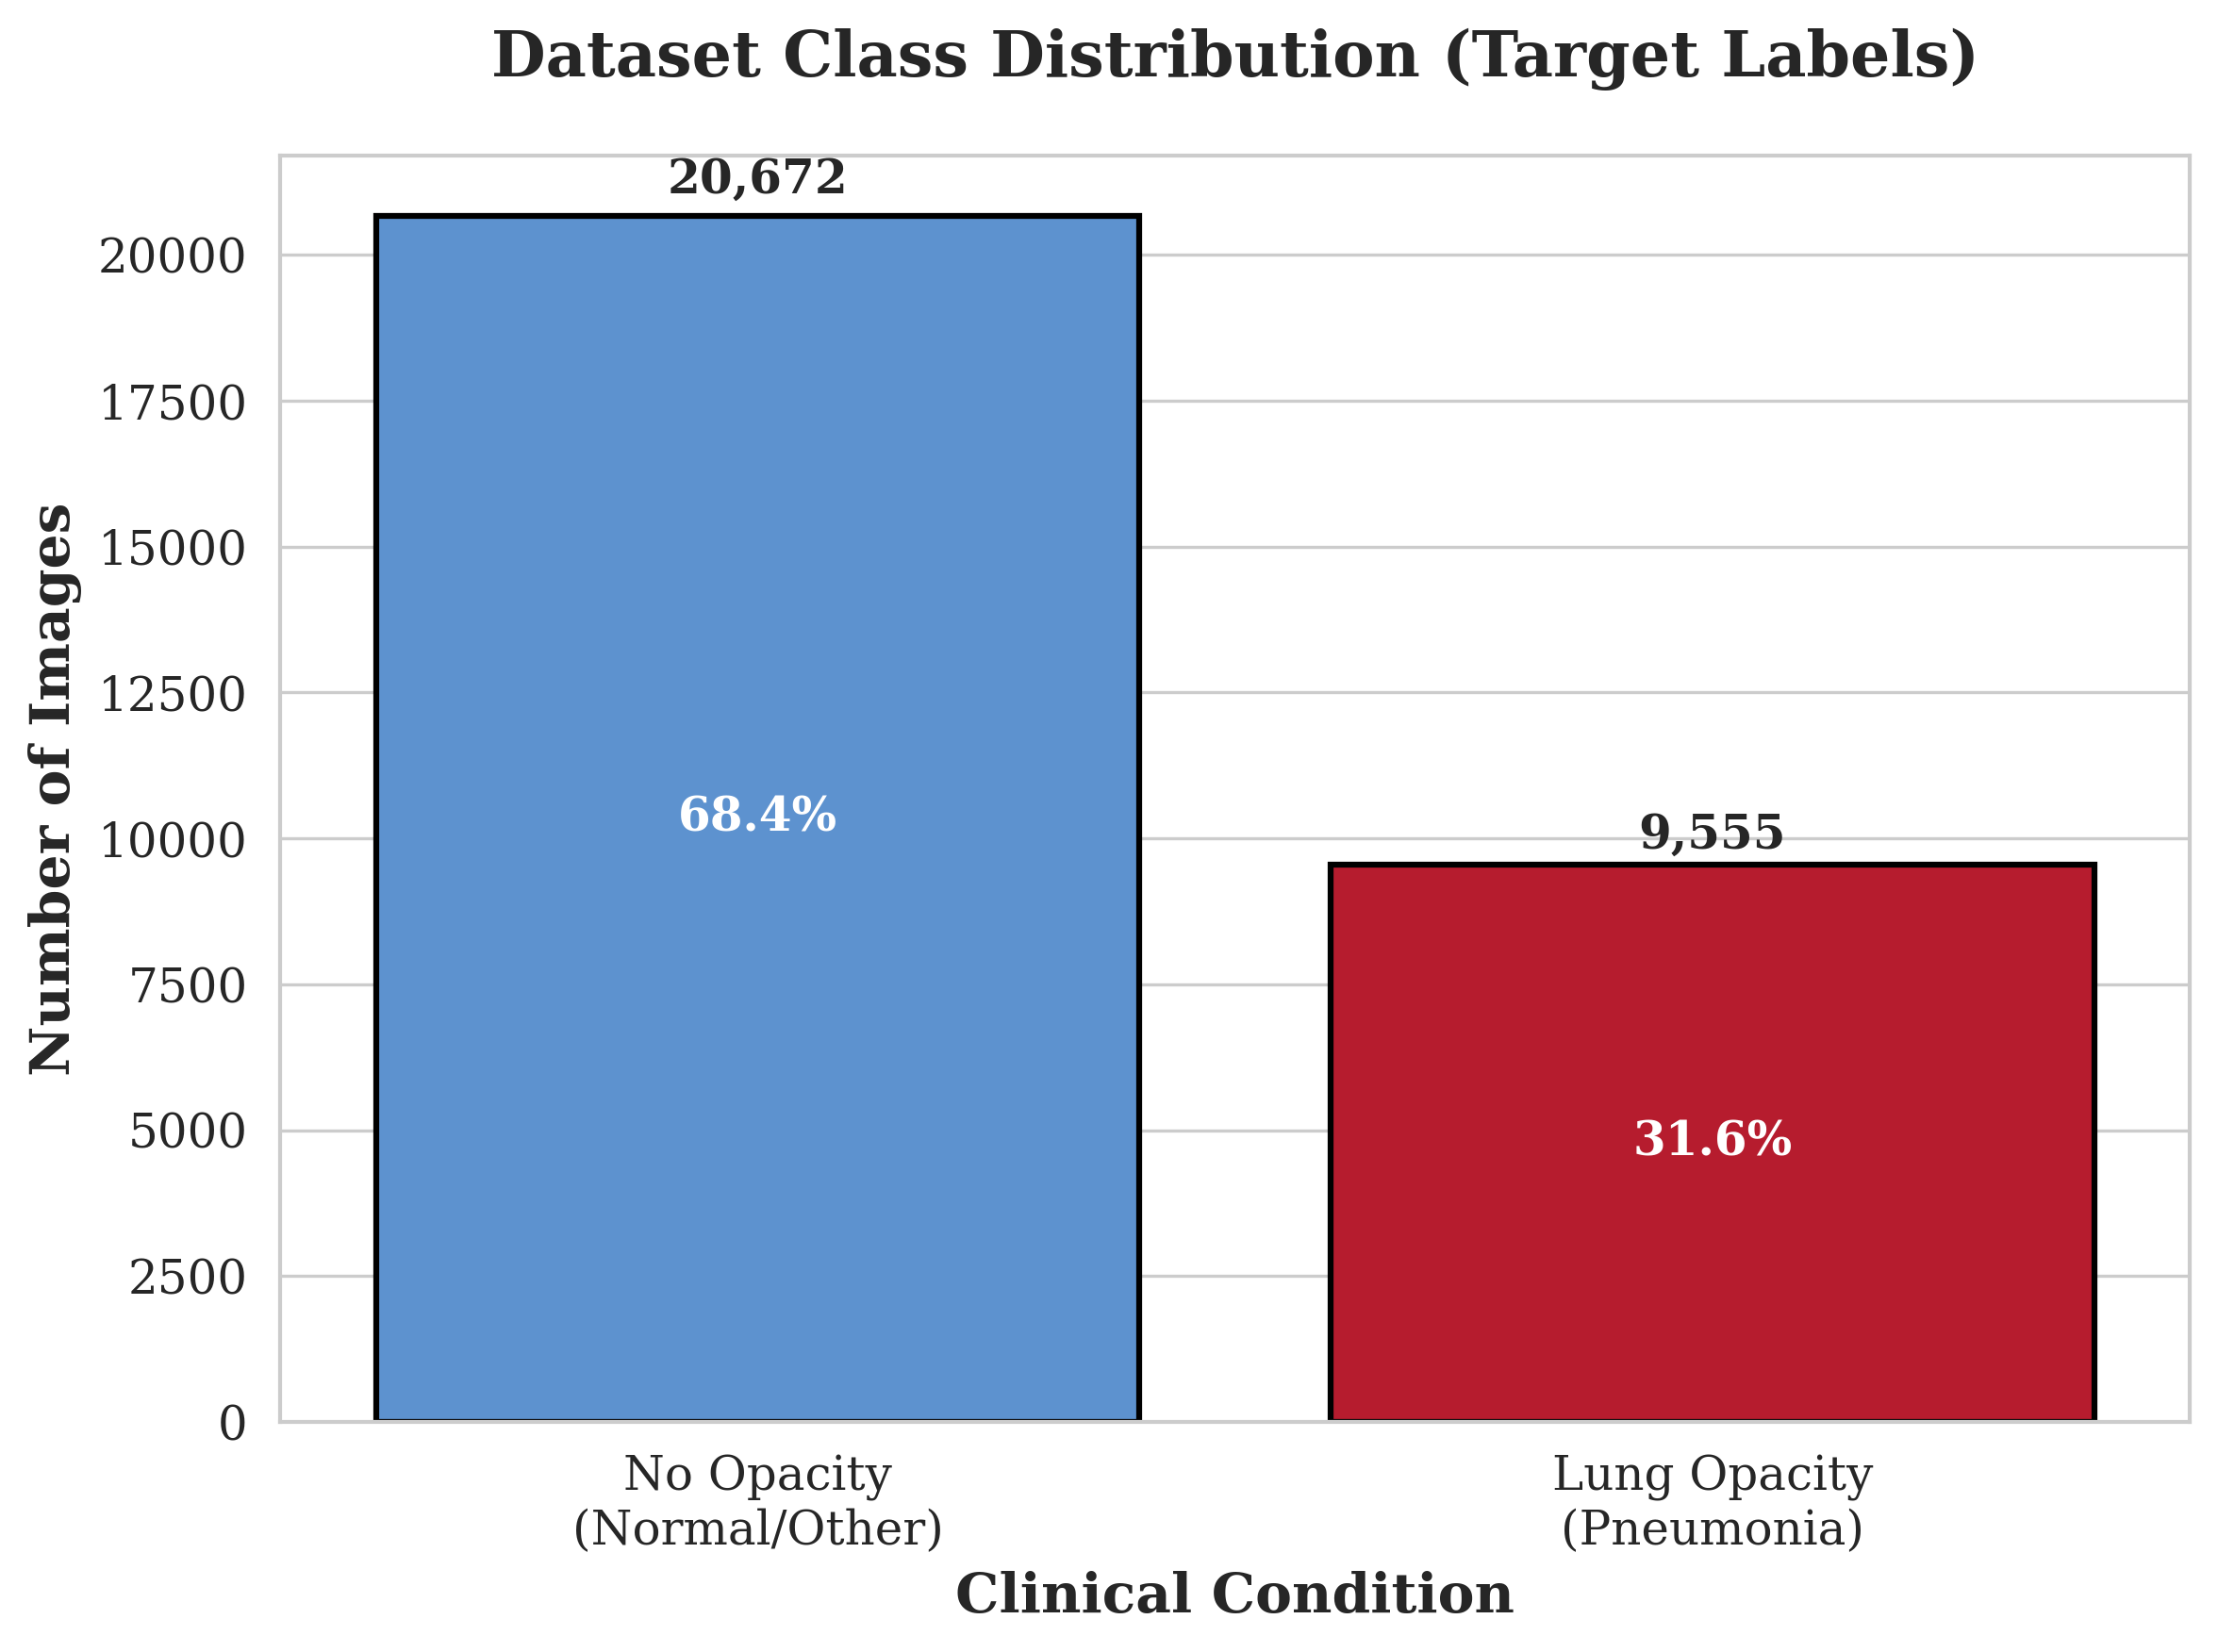
\includegraphics[width=\linewidth]{figs/class_distribution.png}
	\captionof{figure}{Class distribution over the dataset.} 
	\label{fig:class_dis}
\end{minipage}
\vspace{1em}
	
\subsection{Image Pre-processing}
Raw DICOM images were processed using the \texttt{pydicom} library. The pre-processing pipeline consists of the following steps:
\begin{itemize}
	\item \textbf{Resizing:} All images were resized to a fixed resolution of $512 \times 512$ pixels to balance computational efficiency and feature retention.
	\item \textbf{Normalization:} The pixel intensity values were converted to floating-point format and normalized to the range $[0, 1]$ using Min-Max scaling:
	\begin{equation}
		I_{norm} = \frac{I - I_{min}}{I_{max} - I_{min} + \epsilon}
	\end{equation}
	where $\epsilon = 1e^{-8}$ is added for numerical stability.
	\item \textbf{Channel Format:} Since the backbone architecture expects single-channel input for grayscale X-ray images, the inputs were formatted to satisfy that requirement.
\end{itemize}

\subsection{Label Formatting}
For the object detection task, the ground truth bounding boxes were normalized. The original absolute coordinates $(x_{abs}, y_{abs}, w_{abs}, h_{abs})$ were divided by the original image dimensions to obtain relative coordinates in the range $[0, 1]$. In cases where no opacity was present (Target = 0), a dummy bounding box $[0, 0, 0, 0]$ was assigned to maintain consistent tensor dimensions.

\subsection{Data Augmentation}
To improve model generalization and robustness, specifically for the proposed Cellular Neural Network (CeNN) frontend, a robust data augmentation pipeline was applied to the training set using the \texttt{Albumentations}\cite{albumentations} library. The transformations include:
\begin{itemize}
	\item \textbf{Geometric Transformations:} Horizontal Flip (Fig. \ref{fig:hor}) and Shift-Scale-Rotate (Fig. \ref{fig:shift})

 \noindent
 \begin{minipage}{\linewidth}
    \centering
    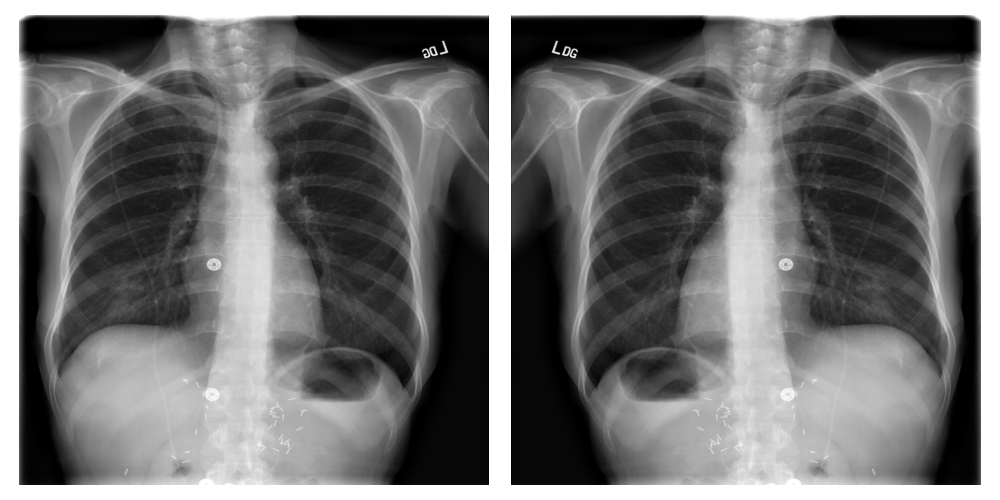
\includegraphics[width=\linewidth]{figs/trasformazioni/result_1_HorizontalFlip_00000514_005.png}
    \captionof{figure}{Horizontal Flip.} % Comando speciale per la didascalia
    \label{fig:hor}
	 \end{minipage}
 \vspace{1em} % Un po' di aria sotto
	
 \noindent
 \begin{minipage}{\linewidth}
    \centering
    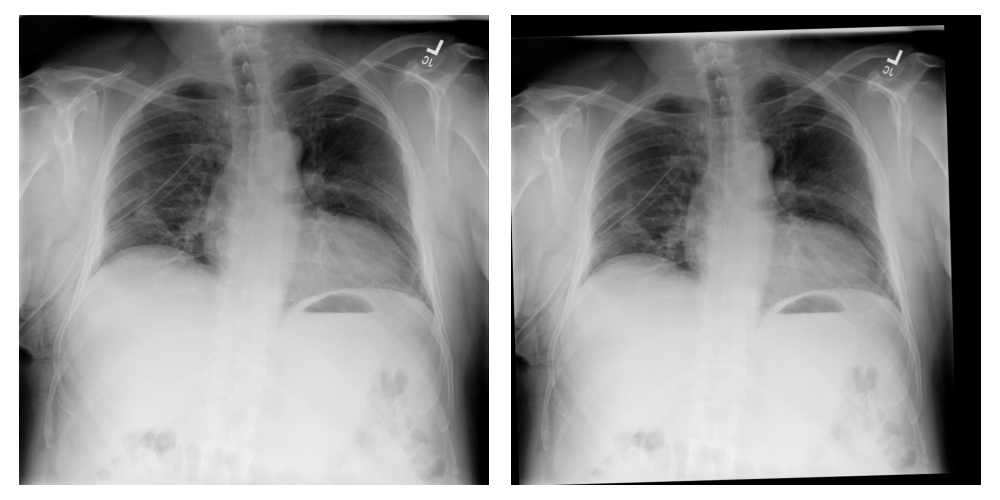
\includegraphics[width=\linewidth]{figs/trasformazioni/result_2_ShiftScaleRotate_00005666_016.png}
    \captionof{figure}{Shift-Scale Rotate.} % Comando speciale per la didascalia
    \label{fig:shift}
	 \end{minipage}
 \vspace{1em} % Un po' di aria sotto
	\item \textbf{Intensity Transformations:} Random Brightness (Fig. \ref{fig:Bright}) and Contrast adjustments (Fig. \ref{fig:contr})
	
 \noindent
 \begin{minipage}{\linewidth}
    \centering
    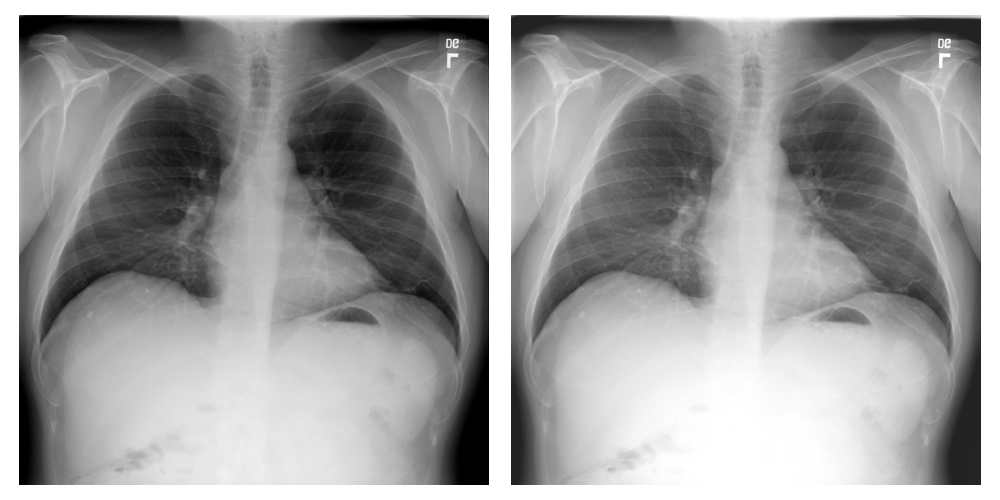
\includegraphics[width=\linewidth]{figs/trasformazioni/result_3_RandomBrightnessContrast_00008027_009.png}
    \captionof{figure}{Random Brightness.} % Comando speciale per la didascalia
    \label{fig:Bright}
	 \end{minipage}
	
 \noindent
 \begin{minipage}{\linewidth}
    \centering
    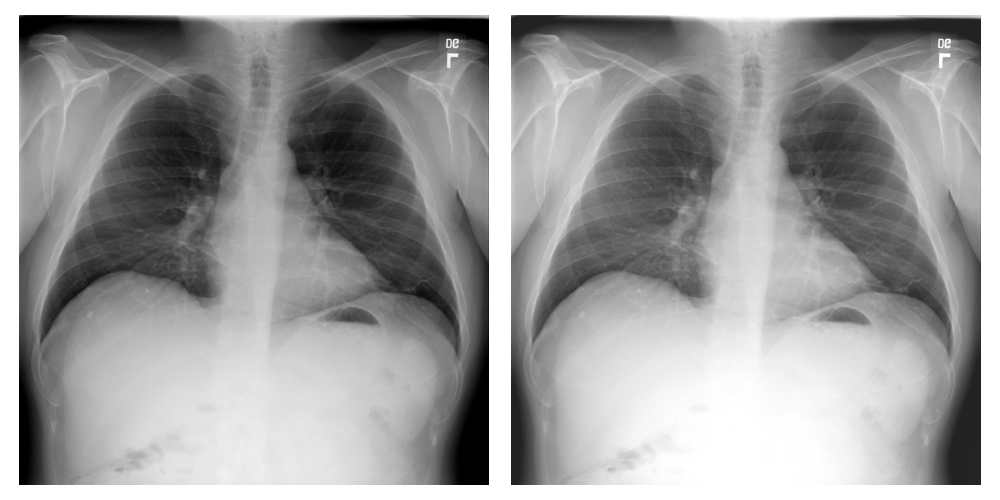
\includegraphics[width=\linewidth]{figs/trasformazioni/result_3_RandomBrightnessContrast_00008027_009.png}
    \captionof{figure}{Contrast adjustment.} % Comando speciale per la didascalia
    \label{fig:contr}
	 \end{minipage}
	
	\item \textbf{Noise Injection:} Gaussian Noise (Fig. \ref{fig:gauss}).
	
 \noindent
 \begin{minipage}{\linewidth}
    \centering
    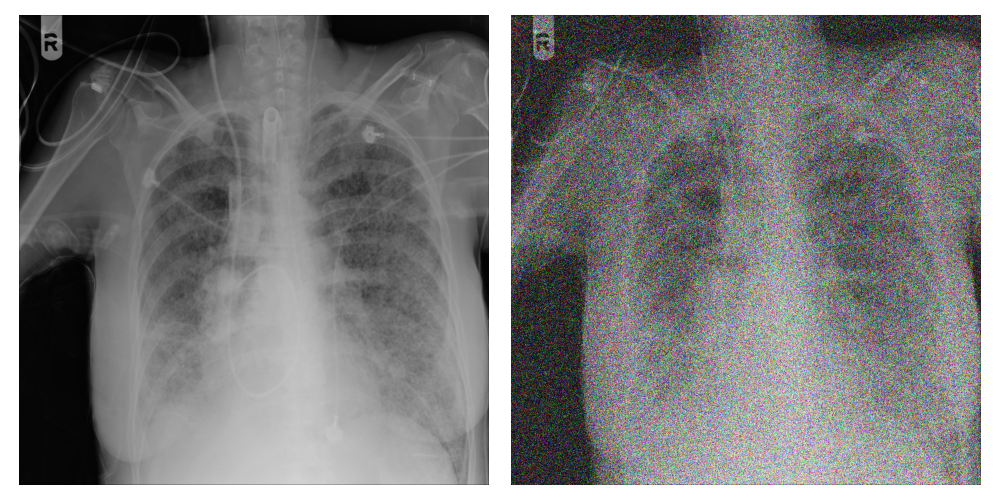
\includegraphics[width=\linewidth]{figs/trasformazioni/result_4_GaussNoise_00001836_050.png}
    \captionof{figure}{Gaussian noise.} % Comando speciale per la didascalia
    \label{fig:gauss}
	 \end{minipage}
	
\end{itemize}
The noise injection steps are particularly relevant to stimulate the dynamic behavior of the CeNN blocks integrated into the model's frontend. The validation set remained unaugmented, undergoing only resizing and normalization.

\section{Proposed Architecture}

The designed system follows a modular pipeline consisting of several distinct stages: the most significant are the CeNN-based pre-processing layer for noise mitigation, the deep convolutional backbone for feature extraction and the multi-head output layer for simultaneous classification and localization.

\noindent
\begin{minipage}{\linewidth}
	\centering
	\includegraphics[width=\linewidth]{figs/schema_rete.png}
	\captionof{figure}{Overview of the proposed architecture.} % Comando speciale per la didascalia
	\label{fig:schema}
\end{minipage}
\vspace{1em} % Un po' di aria sotto

\subsection{Cellular Neural Network (CeNN) Frontend}To enhance the feature extraction capabilities at the initial stage of the pipeline, we utilized an adapted bio-inspired \textit{Cellular Neural Network} (CeNN) module. Unlike standard convolutional layers, this block interprets the feature extraction as the evolution of a dynamic system, effectively capturing global radiographic patterns through continuous-time dynamics approximation.

\subsubsection{Mathematical Formulation}The module's theoretical foundation relies on the state equation proposed by Chua and Yang~\cite{CeNN}. The system is defined by an input $\mathbf{u}$ (the X-ray image), a state $\mathbf{x}$, and an output $\mathbf{y}$. The continuous-time evolution is governed by:$$\frac{d\mathbf{x}(t)}{dt} = -\mathbf{x}(t) + \mathbf{A} \ast \mathbf{y}(t) + \mathbf{B} \ast \mathbf{u} + \mathbf{b}$$where:\begin{itemize}\item $\mathbf{A}$ and $\mathbf{B}$ represent the learnable \textit{feedback} and \textit{feed-forward} templates (convolutional kernels), respectively.\item $\mathbf{b}$ is a learnable bias term broadcasted over the spatial dimensions.\item The output $\mathbf{y}(t)$ is the result of the non-linear activation applied to the state:$$\mathbf{y}(t) = \tanh(\mathbf{x}(t))$$\end{itemize}

\subsubsection{Discrete-Time Implementation}To integrate this dynamic behavior into a standard deep learning pipeline, we implement a discrete-time approximation unrolled over $K$ iterative steps. Unlike traditional approaches that initialize the state to zero, our module initializes the state $\mathbf{x}_0$ by projecting the input space onto the feature space using the feed-forward template:$$\mathbf{x}_0 = \mathbf{B} \ast \mathbf{u}$$For $k = 1, \dots, K$, the state evolution is computed as a weighted interpolation between the previous state (memory) and the current systemic drive:$$\mathbf{x}_k = \alpha \cdot \mathbf{x}_{k-1} + (1 - \alpha) \cdot \left( \mathbf{A} \ast \tanh(\mathbf{x}_{k-1}) + \mathbf{x}_0 + \mathbf{b} \right)$$where $\mathbf{x}_0$ acts as a constant external control signal throughout the integration steps. In our architecture, we empirically set $K=8$.

\subsubsection{Learnable Dynamics and Constraints}We introduced two specific mechanisms to ensure stability, adaptability, and theoretical consistency:
\paragraph{Enforced Bistability}To mimic the saturation behavior of analog CeNN hardware and encourage the emergence of robust, binary-like features, we strictly enforce the bistability criterion. According to standard CeNN theory, a cell is guaranteed to settle into a stable bipolar state if its self-feedback is greater than or equal to $1$. We achieve this by clamping the central spatial weight of the feedback template $\mathbf{A}$ across all channels:$$\mathbf{A}_{c,c} = \max(\mathbf{A}_{c,c}, 1.0)$$where $c$ is the center index of the convolutional kernel. This structural constraint avoids numerical divergence without disrupting the gradient flow for the surrounding weights.
\paragraph{Adaptive Integration Step ($\alpha$)}Instead of utilizing a fixed step size, the integration rate $\alpha$ is modeled as a learnable parameter constrained to the range $(0, 1)$ via a sigmoid activation function:$$\alpha = \sigma(\lambda_{\alpha}) = \frac{1}{1 + e^{-\lambda_{\alpha}}}$$where $\lambda_{\alpha}$ is an optimized logit parameter. This allows the network to automatically learn the optimal trade-off between retaining the memory of the previous state and updating it with the newly computed feedback dynamics.

\subsection{Feature Extraction Backbone}

Following the initial preprocessing by the CeNN module, the refined feature maps are fed into the backbone network. For this study, we employed a \textbf{DenseNet-121} architecture~\cite{densenet}, leveraging the implementation and pre-trained weights provided by the \texttt{torchxrayvision} library~\cite{torchxray}.

\subsubsection{Architecture Justification}
The choice of DenseNet-121 over other architectures (such as ResNet or VGG) is motivated by its specific suitability for medical imaging tasks where training data may be limited compared to natural image datasets. The core concept of DenseNet is the \textit{dense connectivity pattern}: within each dense block, the $l$-th layer receives the feature-maps of all preceding layers, $x_0, \dots, x_{l-1}$, as input:
\begin{equation}
	x_l = H_l([x_0, x_1, \dots, x_{l-1}])
\end{equation}
This architecture offers three critical advantages for pneumonia detection:
\begin{enumerate}
	\item \textbf{Alleviated Vanishing Gradient:} The direct connections to the loss function through the dense blocks facilitate the propagation of gradients, ensuring effective training of deep networks.
	\item \textbf{Feature Propagation and Reuse:} By concatenating features rather than summing them (as in ResNet), the network preserves both low-level features (e.g., bone edges, subtle textures) and high-level semantic information. This is particularly vital for detecting lung opacities, which often present as subtle textural changes.
	\item \textbf{Parameter Efficiency:} DenseNet requires fewer parameters than a ResNet with equivalent depth, reducing the risk of overfitting on the specific RSNA dataset.
\end{enumerate}

\subsubsection{Domain-Specific Transfer Learning}
A key component of our approach is the initialization strategy. Instead of using standard weights pre-trained on ImageNet (natural images), we utilize weights from \texttt{torchxrayvision}, which are pre-trained on a large-scale, heterogeneous aggregation of medical datasets (including NIH ChestX-ray14, CheXpert, MIMIC-CXR, and PadChest). 

This domain-specific transfer learning ensures that the convolutional filters are already tuned to recognize relevant anatomical structures (e.g., ribs, clavicles, lung parenchyma) and pathological textures upon initialization. This leads to faster convergence and significantly improved performance compared to initializing from scratch or using generic natural-image weights, as the "domain gap" between the source and target tasks is minimized.

\subsection{Attention module: CBAM}To further enhance the discriminative power of the features extracted by the DenseNet backbone, we integrated a \textit{Convolutional Block Attention Module} (CBAM)~\cite{cbam} directly after the backbone and before the network branches into the classification and regression heads. While the backbone is effective at extracting hierarchical features, it treats all spatial positions and channels with equal initial importance.In the context of pneumonia detection, however, the relevant information (lung opacities) is often localized in specific regions, while large portions of the image (background, bones, medical devices) act as noise. By applying CBAM as a shared bottleneck, both the classification and the high-resolution regression tasks benefit from sequentially applied attention mechanisms: \textit{Channel Attention} (focusing on "what" to look for) and \textit{Spatial Attention} (focusing on "where" to look).The overall attention process can be summarized as:$$\begin{aligned} \mathbf{F}' &= \mathbf{M}_c(\mathbf{F}) \otimes \mathbf{F} \\ \mathbf{F}'' &= \mathbf{M}_s(\mathbf{F}') \otimes \mathbf{F}' \end{aligned}$$where $\mathbf{F} \in \mathbb{R}^{C \times H \times W}$ is the input feature map, $\mathbf{M}_c$ is the channel attention map, $\mathbf{M}_s$ is the spatial attention map, and $\otimes$ denotes element-wise multiplication.

\subsubsection{Channel Attention Module (CAM)}The Channel Attention Module exploits the inter-channel relationship of the features. Since each channel of a feature map is considered a feature detector, this module learns to assign higher weights to channels that contain meaningful information for the specific pathology.To aggregate spatial information, we employ both \textit{Adaptive Average Pooling} and \textit{Adaptive Max Pooling} to gather distinct spatial descriptors:$$\mathbf{F}_{avg}^c = \text{AvgPool}(\mathbf{F}), \quad \mathbf{F}_{max}^c = \text{MaxPool}(\mathbf{F})$$These descriptors are then forwarded to a shared Multi-Layer Perceptron (MLP), efficiently implemented via $1 \times 1$ convolutions with a reduction ratio to minimize computational overhead, producing the channel attention map:$$\mathbf{M}_c(\mathbf{F}) = \sigma(\text{MLP}(\mathbf{F}_{avg}^c) + \text{MLP}(\mathbf{F}_{max}^c))$$where $\sigma$ represents the sigmoid function. The use of both pooling strategies allows the network to preserve background contextual information while highlighting salient pathological features.

\subsubsection{Spatial Attention Module (SAM)}Following the channel refinement, the Spatial Attention Module focuses on identifying the informative regions within the feature maps. This is crucial for the subsequent localization task, effectively generating a mask that highlights the lungs and suppresses the background.First, we apply average-pooling and max-pooling operations along the channel axis to generate two 2D maps:$$\mathbf{F}_{avg}^s \in \mathbb{R}^{1 \times H \times W}, \quad \mathbf{F}_{max}^s \in \mathbb{R}^{1 \times H \times W}$$These maps are concatenated and convolved with a standard $7 \times 7$ convolution layer, operating without bias, to generate the spatial attention map:$$\mathbf{M}_s(\mathbf{F}') = \sigma(f^{7 \times 7}([\mathbf{F}_{avg}^s; \mathbf{F}_{max}^s]))$$where $f^{7 \times 7}$ represents a convolution operation with a $7 \times 7$ filter size, ensuring a large receptive field to capture contextual spatial relationships.

\subsubsection{Justification for Integration}The inclusion of CBAM as a shared module provides a twofold advantage for our multi-task architecture:
\begin{enumerate}
	\item \textbf{Noise Suppression:} Medical X-rays often contain artifacts and anatomical structures (e.g., clavicles, heart) that can mimic or obscure pneumonia opacities. The adaptive channel rescaling helps the model to ignore irrelevant patterns early in the pipeline.
	\item \textbf{Synergy between Classification and Localization:} Because the spatially refined features ($\mathbf{F}''$) feed both the classification and the regression heads, the Spatial Attention Module acts as a bridge. It leverages the bounding box annotations implicitly during training to guide the classification branch toward the correct pathological regions.
\end{enumerate}

\section{Multi-Task Output Architecture}

To simultaneously address the binary classification task (presence vs. absence of pneumonia) and the localization task (bounding box regression), the proposed architecture diverges into two parallel branches after the feature extraction stage. This design adopts a \textit{Multi-Task Learning} (MTL) strategy, where a shared representation (the backbone + CBAM) is used to solve related tasks.

The rationale behind this choice is twofold:
\begin{enumerate}
	\item \textbf{Computational Efficiency:} By sharing the majority of the parameters (feature extractor), the inference time is significantly lower compared to training two separate models.
	\item \textbf{Feature Regularization:} The localization task acts as an auxiliary supervisor. To accurately predict the bounding box, the backbone is forced to learn spatial features that are strictly correlated with the pathology, thereby reducing the likelihood of the classifier overfitting on background artifacts or confounding factors.
\end{enumerate}

Both heads operate on the refined feature map $\mathbf{F}_{ref} \in \mathbb{R}^{1024 \times H' \times W'}$ output by the CBAM module.

\subsection{Classification Head}
The first branch is dedicated to determining the global probability of pneumonia presence. Since the spatial position of the opacity is irrelevant for the mere detection of the disease in this specific sub-task, we first collapse the spatial dimensions.

The structure consists of the following operations:
\begin{itemize}
	\item \textbf{Global Average Pooling (GAP):} We apply a pooling operation over the spatial dimensions $(H', W')$ to produce a compact feature vector $v \in \mathbb{R}^{1024}$. This aggregates the presence of features regardless of their location:
	\begin{equation}
		v_c = \frac{1}{H' \times W'} \sum_{i=1}^{H'} \sum_{j=1}^{W'} \mathbf{F}_{ref}(c, i, j)
	\end{equation}
	\item \textbf{Fully Connected Layer:} The vector $v$ is fed into a linear transformation layer $f_{cls}: \mathbb{R}^{1024} \to \mathbb{R}^1$, defined by weights $W_{cls}$ and bias $b_{cls}$.
	\item \textbf{Activation:} Finally, a Sigmoid activation function maps the logit to a probability score $p \in [0, 1]$:
	\begin{equation}
		\hat{y}_{cls} = \sigma(W_{cls} \cdot v + b_{cls}) = \frac{1}{1 + e^{-(W_{cls} \cdot v + b_{cls})}}
	\end{equation}
\end{itemize}

\subsection{Localization Head (Regression)}
The second branch is designed to predict the coordinates of the bounding box surrounding the lung opacity. Unlike the classification head, this is formulated as a regression problem.

The head outputs a vector $\mathbf{b} = [x, y, w, h]$, representing the top-left coordinate, width, and height of the box. The process involves:
\begin{itemize}
	\item \textbf{Feature Aggregation:} Similar to the classification head, we employ Global Average Pooling to obtain a feature vector representing the image content.
	\item \textbf{Regression Layer:} A fully connected layer projects the feature vector to a 4-dimensional space: $f_{loc}: \mathbb{R}^{1024} \to \mathbb{R}^4$.
	\item \textbf{Output Normalization:} To ensure the predicted coordinates remain within the valid image boundaries, a Sigmoid activation is applied to the output neurons. This constrains the predictions $\hat{b}$ to the range $[0, 1]$, representing relative coordinates with respect to the image dimensions:
	\begin{equation}
		\hat{\mathbf{b}}_{loc} = \sigma(W_{loc} \cdot v + \mathbf{b}_{loc})
	\end{equation}
	These relative predictions are subsequently mapped back to absolute pixel coordinates during the post-processing phase.
\end{itemize}

\paragraph{Conditional Inference Strategy}
%mettere a posto il testo -----------------------------------
It is important to emphasize that the localization output is functionally dependent on the classification result. Since the regression head continuously predicts candidate coordinates regardless of the image content, a logical gating mechanism is applied during the inference phase. The predicted bounding box $\hat{\mathbf{b}}_{loc}$ is considered valid and retained only if the classification probability $\hat{y}_{cls}$ exceeds a specific decision threshold $\tau$. Conversely, if the model predicts the absence of pneumonia ($\hat{y}_{cls} < \tau$), the regression output is discarded/masked. This strategy effectively eliminates false positive localizations in healthy patients.
	
\subsection{Qualitative Output Analysis}
\label{sec:qualitative_output}

To visually evaluate the performance of the proposed multi-task architecture, sample inference results are presented in Figure \ref{fig:result}.
The visualizations overlay both the true and predicted bounding boxes on the input chest radiographs to demonstrate the model's localization capabilities. The solid green boxes represent the ground truth annotations. The dashed red boxes denote the predicted localizations generated by the network's regression head.

%The first image exemplifies the practical application of the conditional inference strategy. In this instance, the classification head produced a low confidence score (8.9\%) that fell below the established decision threshold $\tau$. Consequently, the regression output was systematically discarded and masked by the gating mechanism, leaving only the ground truth visible. In the subsequent cases, the classification head successfully identified the pathology with high confidence, triggering the localization branch to output the dashed red predictions, which effectively, in two cases out of three, approximate the true opacity regions.
	
\noindent
\begin{minipage}{\linewidth}
	\centering
	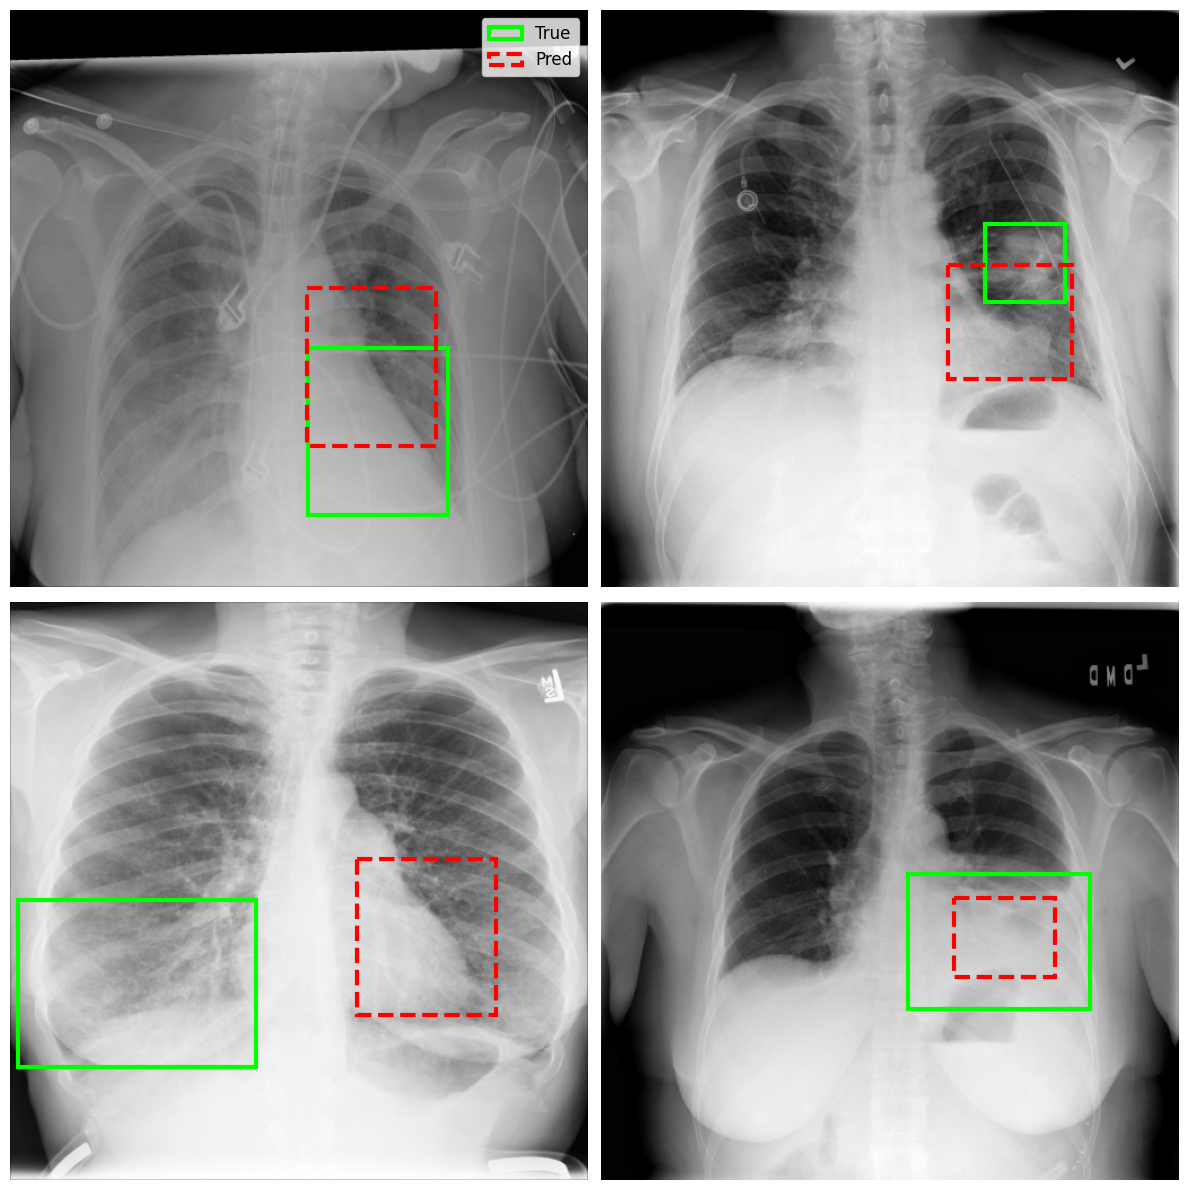
\includegraphics[width=\linewidth]{figs/ris_rete.png}
	\captionof{figure}{Example of results.} % Comando speciale per la didascalia
	\label{fig:result}
\end{minipage}
\vspace{1em} % Un po' di aria sotto
	
\section{Loss Function and Optimization Objective}

Training a multi-task architecture requires a composite objective function that simultaneously minimizes the error for both the binary classification and the bounding box regression. Since the two tasks operate on different scales and semantic levels, simply summing the errors is insufficient. We therefore designed a hybrid loss function that integrates specific weighting and conditional logic.

The total loss $\mathcal{L}_{total}$ is defined as the weighted sum of the classification loss $\mathcal{L}_{cls}$ and the localization loss $\mathcal{L}_{loc}$:

\begin{equation}
	\mathcal{L}_{total} = \lambda_{cls} \cdot \mathcal{L}_{cls} + \lambda_{loc} \cdot \mathcal{L}_{loc}^*
	\label{eq:total_loss}
\end{equation}

where $\lambda_{cls}$ and $\lambda_{loc}$ are hyperparameters used to balance the gradient contribution of each task.

\subsection{Classification Loss ($\mathcal{L}_{cls}$)}
For the detection task (Pneumonia vs. Normal/No Opacity), the objective is to minimize the divergence between the predicted probability distribution and the ground truth. We employ the \textit{Binary Cross-Entropy} (BCE) loss.

Given the ground truth label $y \in \{0, 1\}$ and the predicted probability $\hat{y} \in [0, 1]$, the loss for a single sample is defined as:

\begin{equation}
	\mathcal{L}_{cls}(y, \hat{y}) = - \left[ y \cdot \log(\hat{y}) + (1 - y) \cdot \log(1 - \hat{y}) \right]
\end{equation}

To further address the class imbalance inherent in the RSNA dataset, this loss is often modulated by a weighting factor $\beta$, which assigns a higher penalty to false negatives on the minority class (positive pneumonia cases), ensuring that the model does not converge to a trivial solution (i.e., predicting "healthy" for everyone).

\subsection{Localization Loss - Conditional Masking ($\mathcal{L}_{loc}^*$)}
The localization branch poses a regression problem aimed at minimizing the distance between the predicted bounding box coordinates $\hat{\mathbf{b}} = (\hat{x}, \hat{y}, \hat{w}, \hat{h})$ and the ground truth annotations $\mathbf{b} = (x, y, w, h)$.

For this purpose, we utilize the \textit{Mean Squared Error} (MSE) loss, which penalizes large deviations quadratically:

\begin{equation}
	\mathcal{L}_{MSE}(\mathbf{b}, \hat{\mathbf{b}}) = \frac{1}{4} \sum_{k \in \{x,y,w,h\}} (b_k - \hat{b}_k)^2
\end{equation}

\subsubsection{The Masking Mechanism}
A critical aspect of our training strategy is that the concept of "localization error" is ill-defined for healthy patients (where $y=0$), as there is no ground truth bounding box to regress.
To solve this, we implement a \textit{conditional masking mechanism}. The localization loss is only computed and backpropagated when the ground truth label indicates the presence of opacity. Mathematically, this is expressed by multiplying the regression error by the ground truth class label $y$:

\begin{equation}
	\begin{split}
		\mathcal{L}_{loc}^* &= y \cdot \mathcal{L}_{MSE}(\mathbf{b}, \hat{\mathbf{b}}) \\
		&= \begin{cases} 
			\mathcal{L}_{MSE}(\mathbf{b}, \hat{\mathbf{b}}) & \text{if } y = 1 \text{ (Pneumonia)} \\
			0 & \text{if } y = 0 \text{ (Normal)}
		\end{cases}
	\end{split}
\end{equation}

This formulation ensures that the regression head is trained exclusively on positive samples, preventing the network from hallucinating bounding boxes on healthy images or destabilizing the gradients with undefined target values.

\subsection{Optimization Strategy}
The parameters of the entire network (CeNN frontend, DenseNet backbone, CBAM, and task heads) are optimized end-to-end using the Adam optimizer. The gradients derived from $\mathcal{L}_{total}$ flow back through the bifurcation point, updating the shared feature extractor to learn representations that are beneficial for both recognizing the pathology and defining its spatial boundaries.
	
\section{Semantic Validation via Answer Set Programming (ASP)}
\label{sec:asp_methodology}

While the Deep Learning pipeline described so far excels at extracting texture-based features and identifying patterns, it lacks explicit reasoning capabilities regarding anatomical plausibility and geometric consistency. Neural networks act as statistical black boxes and can often produce "hallucinations", high-confidence False Positives caused by visual artifacts, bone overlaps, or medical devices that resemble opacity textures.

To address this limitation, we integrated a \textit{Semantic Validation Module} based on \textbf{Answer Set Programming (ASP)}. This post-processing layer acts as a "logic filter," accepting or rejecting the predictions of the neural network based on a defined Knowledge Base (KB) of medical and geometric constraints.

\subsection{Neuro-Symbolic Integration Strategy}
The integration follows a Neuro-Symbolic approach where the sub-symbolic system (the CeNN-DenseNet model) acts as a perception engine, and the symbolic system (ASP) acts as a reasoning engine. We utilized \texttt{clingo}\cite{gebser2018multishotaspsolvingclingo}, a potent grounder and solver for logic programs, to implement this bridge directly within the Python pipeline.

The interaction protocol consists of three phases:
\begin{enumerate}
	\item \textbf{Fact Generation:} The raw outputs of the neural network (bounding boxes, confidence scores, and auxiliary metrics like pixel intensity and texture cloudiness) are discretized and converted into logical atoms (facts).
	\item \textbf{Reasoning:} The ASP solver checks these facts against a set of hand-crafted rules (constraints) derived from domain knowledge.
	\item \textbf{Filtering:} The solver returns a stable model indicating whether a prediction is valid or invalid.
\end{enumerate}

Formally, a prediction characterized by geometry $(x, y, w, h)$, statistical confidence $S$, mean intensity $I$, and texture $T$ is mapped to an ASP atom:
\begin{equation}
	\texttt{box(ID, S, X, Y, W, H, I, T).}
\end{equation}

\subsection{Knowledge Base and Logical Constraints}
The core of the module is the logic program that defines what constitutes a "plausible" pneumonia opacity. Throughout our experimental phase, we tested numerous rule configurations. While standard approaches typically employ strict numerical thresholding (e.g., rejecting all predictions where $S < 50$), ASP allows for a more nuanced "weak validation". A bounding box might be rejected despite high confidence if it violates anatomical rules, or accepted with lower confidence if it satisfies strict geometric criteria. 

Among the various configurations tested, we selected two primary logic sets that best balance statistical precision and clinical safety (minimizing False Negatives). 

\subsubsection{Universal Baseline Rules}
Regardless of the specific configuration, all models share a foundational set of Negative Constraints (invalidation rules) to filter out obvious hallucinations:
\begin{itemize}
	\item \textbf{Border and Geometry Artifacts:} Predictions touching the extreme edges of the image (padding artifacts), or exhibiting extreme aspect ratios (perfectly flat or extremely thin lines characteristic of catheters), are strictly rejected.
	\item \textbf{Intensity Anomalies:} Boxes that capture pure black background ($I < 25$) or pure white bone/metal overexposure ($I > 95$) are flagged as invalid.
\end{itemize}

\begin{lstlisting}[language=Prolog]
% Reject edge artifacts and impossible elongations
invalid(ID,"Edge") :-box(ID,_,X,Y,W,H,_,_), X < 5.
invalid(ID,"Flat") :- box(ID,_,_,_,W,H,_,_), W > 4*H.
invalid(ID,"PureWhite") :- box(ID,_,_,_,_,_,I,_), I > 95.
\end{lstlisting}

\subsubsection{Configuration A: Zone-Aware Logic (Smart Heart)}
\label{sec:a_rule}
This configuration introduces spatial awareness, dividing the lung field into specific anatomical zones: the cardiac shadow region (\texttt{zone\_heart}), the upper apex (\texttt{zone\_upper}), and the lower safe areas (\texttt{zone\_lower\_safe}). 

The power of this module lies in its conditional rescue rules. High-confidence predictions ($S \ge 50$) are universally accepted unless flagged by baseline rules. However, sub-threshold predictions are rescued based on their location:
\begin{itemize}
	\item In the \textbf{lower safe zone}, predictions with confidence as low as 28 are validated if they fall within a central safe boundary and possess a normal radiographic intensity.
	\item In the \textbf{heart zone}, the model is more skeptical due to overlapping shadows. A prediction requires a higher confidence ($S \ge 34$) and must explicitly exhibit a "cloudy" texture metric to be considered valid.
\end{itemize}

\begin{lstlisting}[language=Prolog]
% Conditional rescue for the cardiac shadow zone
valid(ID) :- box(ID,S,_,_,_,_,_,_), zone_heart(ID), 
	S >= 34, S < 50, not invalid(ID,_), 
	safe_zone(ID), intensity_ok(ID), is_cloudy(ID).
\end{lstlisting}

\subsubsection{Configuration B: Shape-Based Rescue (Organic)}
\label{sec:b_rule}
This configuration maximizes sensitivity by focusing heavily on biological plausibility rather than specific zones. It introduces the concept of an \texttt{organic} shape—an aspect ratio that is neither a perfect square nor an elongated rectangle, mimicking the amorphous nature of a real lung opacity.

If a low-confidence prediction ($S \ge 32$) exhibits an organic geometry and meets specific size constraints ($W \times H > 2500$), it is rescued. If it lacks an organic shape, it can only be validated if it is strictly located on the safer side and lower regions of the image, where clavicle and medical device artifacts are less prevalent.

\begin{lstlisting}[language=Prolog]
% Define organic shape bounds
is_organic(ID) :- box(ID,_,_,_,W,H,_), 
	10*W < 16*H, 10*H < 16*W.
	
% Rescue organic opacities even with low confidence
valid(ID) :- box(ID,S,_,_,_,_,_), is_organic(ID), 
	S >= 32, S < 50, not invalid(ID,_), 
	safe_zone(ID), intensity_ok(ID), size_ok(ID).
\end{lstlisting}

\subsection{Final Decision Logic}
The final classification for each image is derived using the \textit{Closed World Assumption} (CWA). A prediction is considered an active indicator of pathology only if the solver ultimately labels it as valid.

\begin{lstlisting}[language=Prolog]	
% Final Image Classification
has_pneumonia :- valid(ID).
\end{lstlisting}
	
\section{Training Methodology}

The training of a complex, multi-task architecture operating on high-resolution medical images presents significant optimization and hardware challenges. This section details the training regime, including the data handling recap, the transfer learning strategy, and the techniques employed to ensure stable convergence under memory constraints.

\subsection{Data Setup and Regularization}
As detailed in previous sections, the dataset was partitioned into an 80:20 train-validation split. To counteract the severe class imbalance (prevalence of healthy patients), a \texttt{WeightedRandomSampler} was employed during the DataLoader construction, ensuring that each mini-batch contained a balanced representation of both positive and negative samples. 

Furthermore, robust data augmentation techniques were applied exclusively to the training set. Alongside standard geometric and intensity transformations, specific noise injection techniques (Gaussian Noise and Blur) were introduced. This noise acts as a critical regularizer and serves the specific purpose of stimulating the dynamic temporal evolution of the CeNN frontend, preventing the continuous-time solver from collapsing into trivial identity mappings.

\subsection{Transfer Learning and Layer Freezing Strategy}
\label{sec:transf_learn}
To leverage the rich feature representations learned from large-scale medical datasets, the DenseNet-121 backbone was initialized with pre-trained weights from the \texttt{torchxrayvision} library. However, updating all parameters of the network simultaneously from the first epoch can lead to catastrophic forgetting, where the pre-trained weights are destroyed by the initially large and noisy gradients propagating from the randomly initialized custom heads (CeNN and MTL heads).

To mitigate this, we employed a \textit{partial layer freezing} strategy:
\begin{itemize}
	\item \textbf{Frozen Backbone:} During the initial training phase, the gradients for the first set of dense blocks in the backbone were disabled (\texttt{requires\_grad = False}). These early layers typically detect generic low-level features (e.g., edges, bone structures) which are universally applicable across different radiographic datasets.
	\item \textbf{Active Modules:} The custom CeNN frontend, the CBAM module, the final layers of the DenseNet, and the two output heads (Classification and Localization) were left active (\texttt{requires\_grad = True}).
\end{itemize}
This setup forces the network to adapt the new modules to the existing robust feature representations. Once the custom heads have converged to a stable state, the backbone can be partially or fully unfrozen for a final \textit{fine-tuning} phase with a significantly reduced learning rate, allowing the entire system to synergistically adapt to the specific RSNA dataset.

\subsection{Gradient Accumulation and Virtual Batch Size}
Processing high-resolution medical images (e.g., $512 \times 512$ pixels) using a deep architecture like DenseNet combined with a computationally intensive CeNN frontend requires substantial GPU memory (VRAM). This memory constraint typically forces the use of very small physical batch sizes.

However, training with very small batches leads to extremely noisy gradient estimates, which can destabilize the optimization process and degrade the performance of layers that rely on batch statistics, such as Batch Normalization.

To overcome this hardware limitation without sacrificing model stability, we implemented \textbf{Gradient Accumulation}. Instead of updating the network weights after every forward pass, the gradients are accumulated (summed) over multiple iterations. The optimizer step is only performed after $A$ accumulation steps.

Mathematically, if $B_{phys}$ is the physical batch size that fits in VRAM, the \textit{Virtual Batch Size} $B_{virt}$ is defined as:
\begin{equation}
	B_{virt} = B_{phys} \times A
\end{equation}
For instance, using a physical batch of 4 and accumulating gradients for 8 steps yields an effective virtual batch size of 32. The update rule for the network parameters $\theta$ at step $t$ becomes:
\begin{equation}
	\theta_{t+1} = \theta_t - \eta \cdot \nabla_\theta \left( \frac{1}{A} \sum_{i=1}^{A} \mathcal{L}_{total}^{(i)} \right)
\end{equation}
where $\eta$ is the learning rate and $\mathcal{L}_{total}^{(i)}$ is the loss of the $i$-th physical mini-batch. This technique perfectly simulates the training dynamics of a large batch size, providing smooth and reliable gradient directions for the optimizer.

\subsection{Optimization and Learning Rate Scheduling}
The active parameters were optimized using the \textbf{Adam} (Adaptive Moment Estimation) optimizer. Adam was chosen for its ability to compute individual adaptive learning rates for different parameters from estimates of first and second moments of the gradients, which is particularly beneficial for architectures containing heterogeneous modules (like the recurrent-like CeNN and the standard convolutional DenseNet).

To further stabilize training, we coupled the optimizer with a learning rate scheduler,  the \texttt{ReduceLROnPlateau} strategy. The scheduler monitors the validation classification loss ($\mathcal{L}_{cls}$) at the end of each epoch. If the metric stops improving for a defined number of consecutive epochs (\textit{patience}), the learning rate is reduced by a predefined factor. This approach allows the model to make large weight updates during the early stages of training and progressively fine-tune the parameters as it approaches a local minimum, effectively preventing oscillations and overshooting.

\subsection{Training Convergence and Stability}
To empirically validate the proposed two-phase optimization strategy and the layer freezing schedule (discussed in Section \ref{sec:transf_learn}), we continuously monitored the total composite loss ($\mathcal{L}_{total}$) during both the training and validation phases. As illustrated in Figure \ref{fig:loss_curve}, the decoupled training approach proved highly effective.

\noindent
\begin{minipage}{\linewidth}
	\centering
	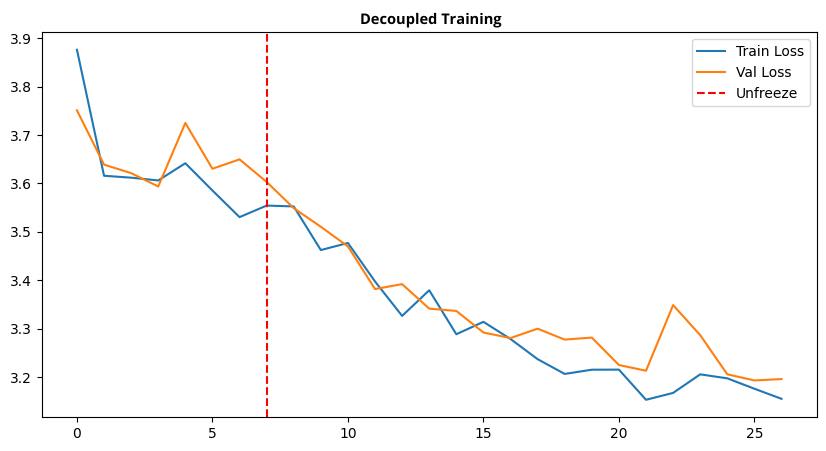
\includegraphics[width=\linewidth]{figs/loss_curve_final.png} % Assicurati di rinominare l'immagine o cambiare il path
	\captionof{figure}{Training and validation loss curves over the epochs. The red dashed line marks the "Unfreeze" point, transitioning from the warmup phase (frozen backbone) to full-network fine-tuning.}
	\label{fig:loss_curve}
\end{minipage}
\vspace{1em}

During the initial warmup phase (prior to the unfreeze point), the validation loss steadily decreases as the newly initialized custom modules (CeNN frontend, CBAM, and MTL heads) adapt to the robust feature representations of the frozen DenseNet backbone. Once these external layers reach a stable state, the entire network is unfrozen for end-to-end fine-tuning. 

Crucially, the graph demonstrates that the unfreezing event does not trigger sudden loss spikes or catastrophic forgetting, a common failure mode in transfer learning. Thanks to the carefully scaled learning rate and the prior stabilization of the top layers, both the training and validation losses continue to converge smoothly. The tight correlation between the two curves throughout the entire training process confirms optimal generalization and the absence of overfitting on the highly imbalanced RSNA dataset.

\section{Results and Evaluation}

\subsection{Deep Learning Pipeline Performance and Threshold Optimization}
To establish a robust baseline for the proposed architecture, we first evaluated the network's classification capabilities prior to any logical post-processing. Given the inherent class imbalance of the dataset, relying solely on standard accuracy at a default decision boundary can be misleading. Therefore, during the evaluation phase, Test-Time Augmentation (TTA) was strictly employed. TTA enhances the reliability of the predictions by averaging the outputs of the original image and its horizontally flipped counterpart, reducing variance and stabilizing the spatial feature representation against patient misalignments.

Coupled with TTA, an extensive threshold optimization search was conducted on a validation subset to maximize the F1-Score and find the optimal balance between Precision and Recall.

\begin{table}[htbp]
	\centering
	\caption{Threshold optimization search on the validation subset. The threshold of 0.4 provides the best F1-Score and a strong Recall, making it optimal for medical screening.}
	\label{tab:thresh_search}
	\begin{tabular*}{\linewidth}{@{\extracolsep{\fill}} c c c c c @{}}
		\toprule
		\textbf{Threshold} & \textbf{Precision} & \textbf{Recall} & \textbf{F1-Score} & \textbf{False Positives} \\
		\midrule
		0.20 & 0.4395 & 0.8845 & 0.5873 & 1386 \\
		0.30 & 0.4919 & 0.8177 & 0.6143 & 1038 \\
		\textbf{0.40} & \textbf{0.5408} & \textbf{0.7282} & \textbf{0.6207} & \textbf{760} \\
		0.50 & 0.6331 & 0.6037 & 0.6181 & 430 \\
		0.60 & 0.7555 & 0.3344 & 0.4636 & 133 \\
		0.70 & 0.9167 & 0.0448 & 0.0853 & 5 \\
		\bottomrule
	\end{tabular*}
\end{table}

As demonstrated in the validation analysis (Table \ref{tab:thresh_search}), lowering the decision boundary from the default 0.5 to an optimal threshold of 0.4 yielded the best overall F1-Score. To fully assess the clinical impact of this tuning, we compared the inference results on the broader dataset using both the default 0.5 threshold and the optimized 0.4 threshold.

\noindent
\begin{minipage}{\linewidth}
	\centering
	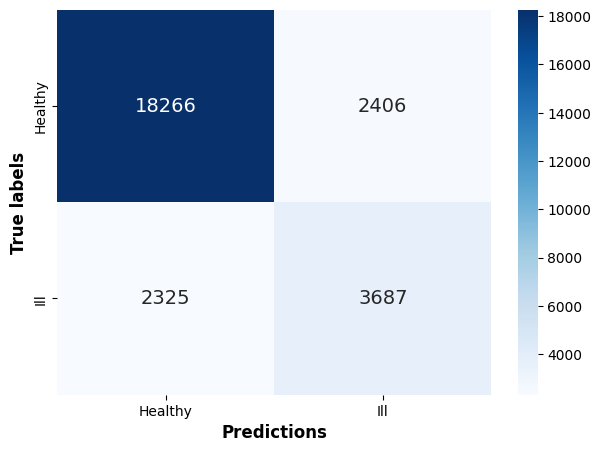
\includegraphics[width=\linewidth]{figs/risultati.png}
	\captionof{figure}{Confusion Matrix evaluated with the default 0.5 classification threshold.}
	\label{fig:risultati_05}
\end{minipage}
\vspace{1em}

\noindent
\begin{minipage}{\linewidth}
	\centering
	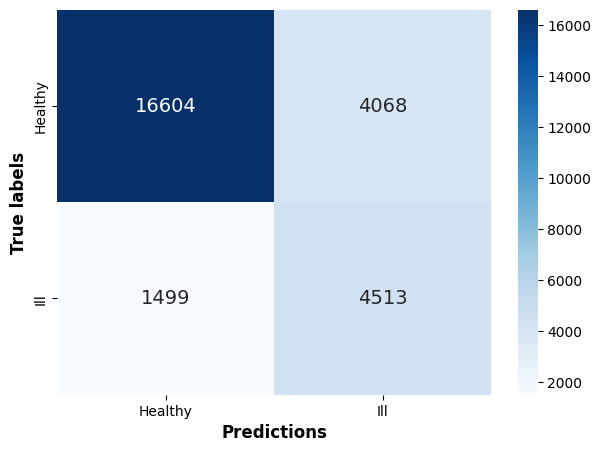
\includegraphics[width=\linewidth]{figs/risultati_0.4.png}
	\captionof{figure}{Confusion Matrix evaluated with the optimized 0.4 classification threshold.}
	\label{fig:risultati_04}
\end{minipage}
\vspace{1em}

The comparison between Figure \ref{fig:risultati_05} and Figure \ref{fig:risultati_04} dictates a clear choice for the remainder of the project. At the standard 0.5 threshold, the network successfully identifies 3,687 True Positives but misses 2,325 cases (False Negatives). By shifting the threshold to 0.4, the model inherently favors Recall over Precision. The True Positives rise significantly to 4,513, safely dropping the False Negatives down to 1,499. 

This adjustment is particularly crucial in a medical screening context. In clinical practice, maximizing Sensitivity (Recall) is paramount to ensure that potentially life-threatening conditions are not overlooked. A False Negative carries catastrophic clinical consequences, whereas a False Positive merely results in a secondary review by a radiologist. Consequently, the 0.4 threshold, which minimizes missed diagnoses despite an unavoidable increase in False Positives (from 2,406 to 4,068), is definitively selected as the optimal sub-symbolic baseline. The subsequent Answer Set Programming (ASP) logic layer is specifically engineered to contextualize and filter out these excess False Positives later in the pipeline.


\subsection{Localization Accuracy and Metric Recontextualization}

While the primary focus of the neural pipeline is to establish a reliable binary classification, the multi-task architecture simultaneously performs bounding box regression to generate spatial priors for the subsequent Semantic Validation Module (ASP).

Evaluating the raw localization output on True Positive cases yielded a Mean Intersection over Union (IoU) of 0.0817 and a Centroid Euclidean Distance (Mean Pixel Error) of 40.7 pixels. In standard natural image tasks, an IoU below 0.5 is typically considered a failure. However, applying strict IoU thresholds to radiographic opacities is methodologically flawed. Pneumonia presents as a highly diffuse, semi-transparent cloud lacking sharp boundaries. Furthermore, ground truth annotations in the RSNA dataset frequently consist of overly large bounding boxes drawn by radiologists to encompass broad suspicious regions. If the regression head predicts a tightly bounded box strictly localized over the highest-density core of the opacity, the IoU mathematically collapses due to the large union area, despite the prediction being clinically highly accurate.

By shifting the evaluation from boundary overlap (IoU) to focal point proximity (Centroid Euclidean Distance), the system's actual reliability emerges. A mean deviation of 40.7 pixels on a 512$\times$512 high-resolution radiograph represents an error margin of less than 8\%. This demonstrates that while the network does not delineate the exact contours of the diffuse pathology, it successfully and consistently pinpoints its anatomical center. This focal localization provides exactly the necessary, reliable spatial coordinates required by the neuro-symbolic logic layer to evaluate regional plausibility.

\subsection{Impact of Semantic Validation (Neuro-Symbolic ASP)}
In the previous sections, we demonstrated that lowering the global decision threshold to 0.4 improves Sensitivity (Recall) by blindly accepting lower-probability predictions. However, a blanket threshold reduction is a purely statistical intervention that lacks medical context. To achieve a more intelligent, context-aware triage, the Answer Set Programming (ASP) Semantic Validation Module is applied directly to the raw network predictions evaluated at the standard 0.5 decision boundary.

The rationale for establishing the 0.5 threshold as the baseline for the reasoning engine is fundamental to the neuro-symbolic approach. Predictions with a confidence score $\ge 0.5$ are considered "high-confidence" and are universally accepted by the ASP module, provided they do not violate foundational geometric rules (e.g., edge artifacts). Conversely, predictions falling below this 0.5 threshold are not discarded. Instead, they are passed to the ASP solver for a potential "intelligent rescue". The logic conditionally rescues these sub-threshold predictions only if they satisfy strict anatomical, spatial, and geometric axioms defined in the Knowledge Base. 

During our experimental phase, we evaluated two primary ASP configurations that successfully operationalize this clinical priority.

\subsubsection{Configuration A: Zone-Aware Logic (Smart Heart)}
The first selected configuration (detailed in \ref{sec:a_rule}) represents an optimal sweet spot between maintaining high statistical precision and enhancing clinical safety. The logic in this module introduces context-aware thresholds based on distinct anatomical zones, such as the cardiac shadow region or the lower lung boundaries, paired with specific intensity metrics.

\noindent
\begin{minipage}{\linewidth}
	\centering
	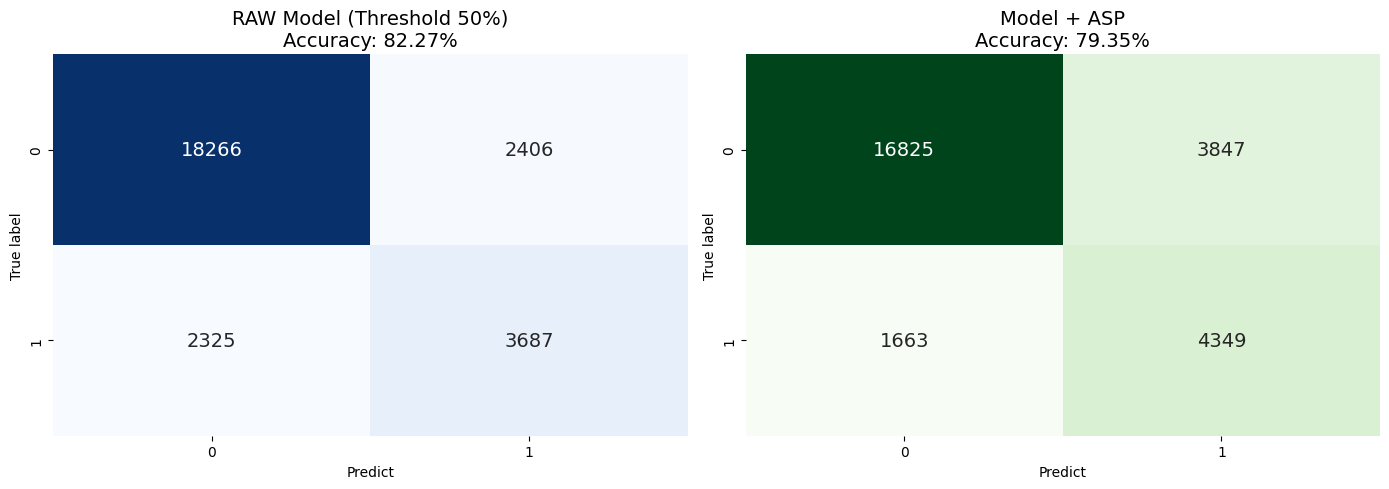
\includegraphics[width=\linewidth]{figs/conf_matr_asp/Conf_20.png}
	\captionof{figure}{Performance of the Zone-Aware (Smart Heart) ASP configuration compared to the raw neural network at the baseline 0.5 threshold.}
	\label{fig:asp_smart_heart}
\end{minipage}
\vspace{1em}

As shown in Figure \ref{fig:asp_smart_heart}, the raw neural network operating at a 0.5 threshold misses 2,325 pneumonia cases (False Negatives). By applying the semantic rules, the logic solver successfully recovers predictions that the neural network had assigned low confidence to, provided they make anatomical sense in their respective zones. This targeted intervention rescues 662 true pneumonia cases, reducing the False Negatives down to 1,663. While the inclusion of lower-confidence boxes inevitably increases the False Positives (dropping global accuracy slightly to 79.35\%), this configuration successfully corrects the network's anatomical blind spots without severely degrading the system's overall statistical reliability.

\subsubsection{Configuration B: Shape-Based Rescue (Organic)}
For triage environments where Sensitivity (Recall) is the absolute priority, we evaluated the "Organic" configuration. As explained in Section \ref{sec:b_rule} this rule set is heavily biased towards biological plausibility, evaluating whether a low-confidence prediction possesses an organic aspect ratio (rejecting perfect squares or unusually thin artifacts like catheters) and whether it falls within the safe boundaries of the lung cavities.

\noindent
\begin{minipage}{\linewidth}
	\centering
	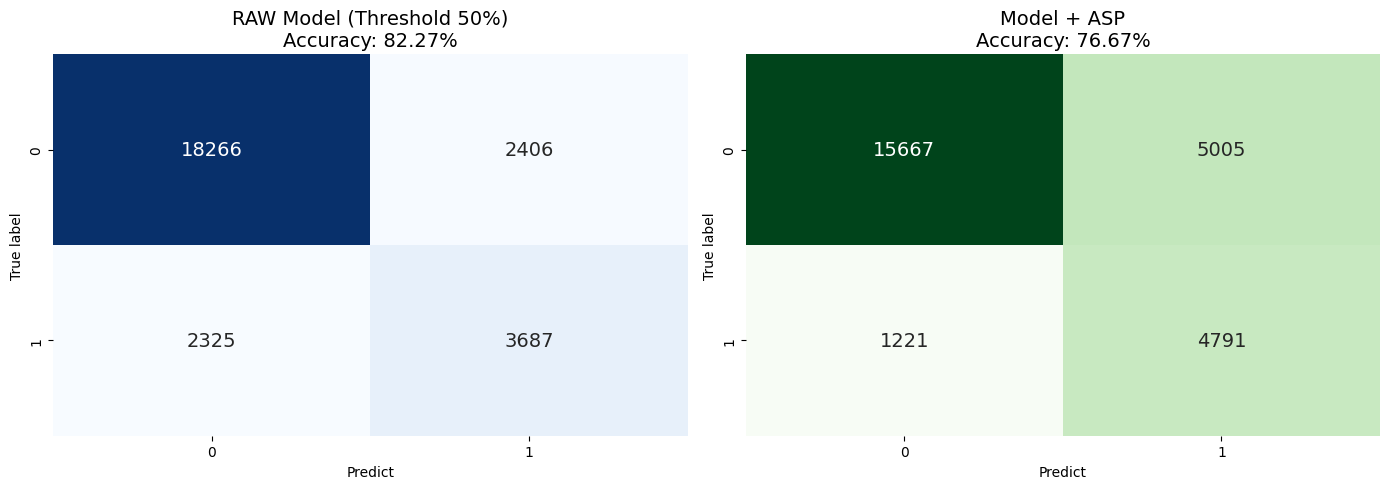
\includegraphics[width=\linewidth]{figs/conf_matr_asp/Conf_29.png}
	\captionof{figure}{Performance of the Shape-Based (Organic) ASP configuration. Prioritizing biological shape plausibility drastically reduces False Negatives.}
	\label{fig:asp_organic}
\end{minipage}
\vspace{1em}

Figure \ref{fig:asp_organic} illustrates the drastic clinical impact of this approach. The organic logic nearly halves the number of False Negatives, dropping them from the baseline 2,325 down to an impressive 1,221. By forcing the system to trust biologically plausible shapes even when the statistical confidence is weak, 1,104 true pneumonia cases are saved. The trade-off is a further reduction in global Accuracy (76.67\%) and an increase in False Positives (5,005). 

However, from a medical standpoint, this specific operational mode is highly desirable. It configures the AI as an ultra-conservative screening tool that flags any geometrically valid anomaly for human review, dramatically minimizing the risk of discharging a patient with an undetected pathology.


\begin{table*}[htbp]
	\centering
	\caption{Comprehensive performance comparison across different classification strategies on the full test dataset. The Neuro-Symbolic (Organic) approach maximizes Recall and minimizes False Negatives, making it the safest configuration for clinical screening.}
	\label{tab:master_results}
	\begin{tabular*}{\linewidth}{@{\extracolsep{\fill}} l c c c c c c @{}}
		\toprule
		\textbf{Configuration} & \textbf{Accuracy} & \textbf{Precision} & \textbf{Recall} & \textbf{F1-Score} & \textbf{FN} & \textbf{FP} \\
		\midrule
		RAW Model (Thresh 0.5) & \textbf{82.27\%} & \textbf{0.605} & 0.613 & 0.609 & 2325 & \textbf{2406} \\
		TTA Optimized (Thresh 0.4) & 79.14\% & 0.526 & 0.751 & \textbf{0.618} & 1499 & 4068 \\
		\midrule
		ASP Logic (Smart Heart) & 79.35\% & 0.531 & 0.723 & 0.612 & 1663 & 3847 \\
		ASP Logic (Organic) & 76.67\% & 0.489 & \textbf{0.797} & 0.606 & \textbf{1221} & 5005 \\
		\bottomrule
	\end{tabular*}
\end{table*}

\section{Comparative Analysis and Noise Robustness Benchmarking}
\label{sec:comparative_analysis}

Visual localization and robust image recognition in unstructured or medical environments remain significant challenges due to the performance degradation of standard Convolutional Neural Networks (CNNs) under noise, low lighting, or artifacts. To rigorously validate the noise-suppression capabilities of the proposed Cellular Neural Network (CeNN) frontend, we conducted a comprehensive comparative analysis. This section benchmarks the proposed hybrid architecture against both its raw backbone and several state-of-the-art deep learning models under increasing levels of Gaussian noise.

\subsection{Evaluated Architectures and Training Setup}
To establish a robust and fair baseline, the proposed hybrid architecture was benchmarked against several state-of-the-art deep learning models widely used in image classification:
\begin{itemize}
	\item \textbf{DenseNet-121 (Ablation Baseline)}: The isolated backbone used in our pipeline, without the CeNN frontend.
	\item \textbf{ResNet (Standard)}: The foundational Residual Network \cite{he2016deep}.
	\item \textbf{SE-ResNet}: An evolution of ResNet incorporating Squeeze-and-Excitation (SE) blocks for channel-wise attention \cite{hu2018squeeze}.
	\item \textbf{EfficientNet-B0}: A modern architecture \cite{tan2019efficientnet} utilizing compound scaling for optimized efficiency.
	\item \textbf{Proposed Hybrid CeNN}: Our integrated architecture featuring the CeNN frontend.
\end{itemize}

A critical distinction regarding the initialization and training protocol must be noted. To simulate a standard development workflow, all comparison models (ResNet, SE-ResNet, and EfficientNet) were initialized with standard weights pre-trained on the ImageNet dataset. Subsequently, to ensure a fair comparison of their learning capacity, every model was fine-tuned on the same RSNA Pneumonia Detection dataset using the identical training-validation split and balancing strategies described in Section \ref{sec:dataset}

When analyzing these models, a critical architectural distinction must be made. ResNet, SE-ResNet, and EfficientNet-B0 act as dedicated single-task classifiers. In contrast, the proposed architecture employs a Multi-Task Learning (MTL) strategy, simultaneously performing binary classification and high-resolution bounding box regression. Solving two complex spatial and semantic tasks with a shared feature extractor introduces a heavier optimization burden. However, this dual capability makes the proposed system significantly more valuable for clinical triage.

\subsection{Experimental Setup}
The noise robustness evaluation was conducted on a representative, balanced subset of the test set. This choice was necessitated by the high computational cost of performing inference across five different architectures, each subjected to six progressive levels of Gaussian noise (0\%, 15\%, 30\%, 45\%, 60\%, and 90\% variance limits). 

The models were evaluated on their classification accuracy under these corrupted conditions to measure structural resilience. Detailed confusion matrices for all evaluated models across the entire noise spectrum, along with the exact numerical results, are provided in Appendix \ref{sec:appendix_matrices} (see Table \ref{tab:noise_accuracy} and Figure \ref{fig:noise_comparison_p1}).

\begin{note}
	Due to the different scale of the evaluation set, the baseline metrics (0\% noise) reported in this comparative analysis may show slight numerical variations compared to the results obtained on the full RSNA dataset reported in Section \ref{sec:asp_methodology}. However, the subset remains statistically consistent, ensuring the validity of the observed performance degradation curves.
\end{note}


This experimental design allows us to observe not only the peak performance in ideal conditions but also the "rate of decay" of each architecture. By training all models on the same data, we ensure that any observed robustness is a direct result of the architectural components (such as the CeNN frontend or SE blocks) rather than differences in data exposure.

\subsection{Results and Discussion}
The comparative performance degradation across all noise levels is visually synthesized in Figure \ref{fig:noise_line_chart}.

At baseline conditions (0\% noise), highly parameterized single-task architectures naturally exhibit superior accuracy. EfficientNet-B0 and standard ResNet achieve 87.2\% and 86.0\% respectively, outperforming the proposed CeNN hybrid model (79.5\%). This initial gap is expected given the multi-task nature of our network.

However, as signal corruption increases, the structural limitations of standard CNNs become clearly visible. The ablation baseline (DenseNet Without CeNN) experiences a catastrophic structural collapse at extreme noise levels (90\%), dropping to an accuracy of 29.8\%. Standard ResNet also degrades significantly, falling to 67.8\%. 

Conversely, SE-ResNet and EfficientNet-B0 demonstrate strong inherent resilience, maintaining accuracies above 81\% even at extreme noise levels.

Most notably, the proposed CeNN architecture exhibits a highly resilient degradation curve. While starting at a lower baseline accuracy due to the MTL constraint, the network only loses 6.2\% accuracy across the entire noise spectrum (dropping from 79.5\% to 73.3\%). The CeNN layer acts as an exceptional deterministic filter, preventing severe degradation and maintaining stable feature extraction regardless of signal corruption.

\noindent
\begin{minipage}{\linewidth}
	\centering
	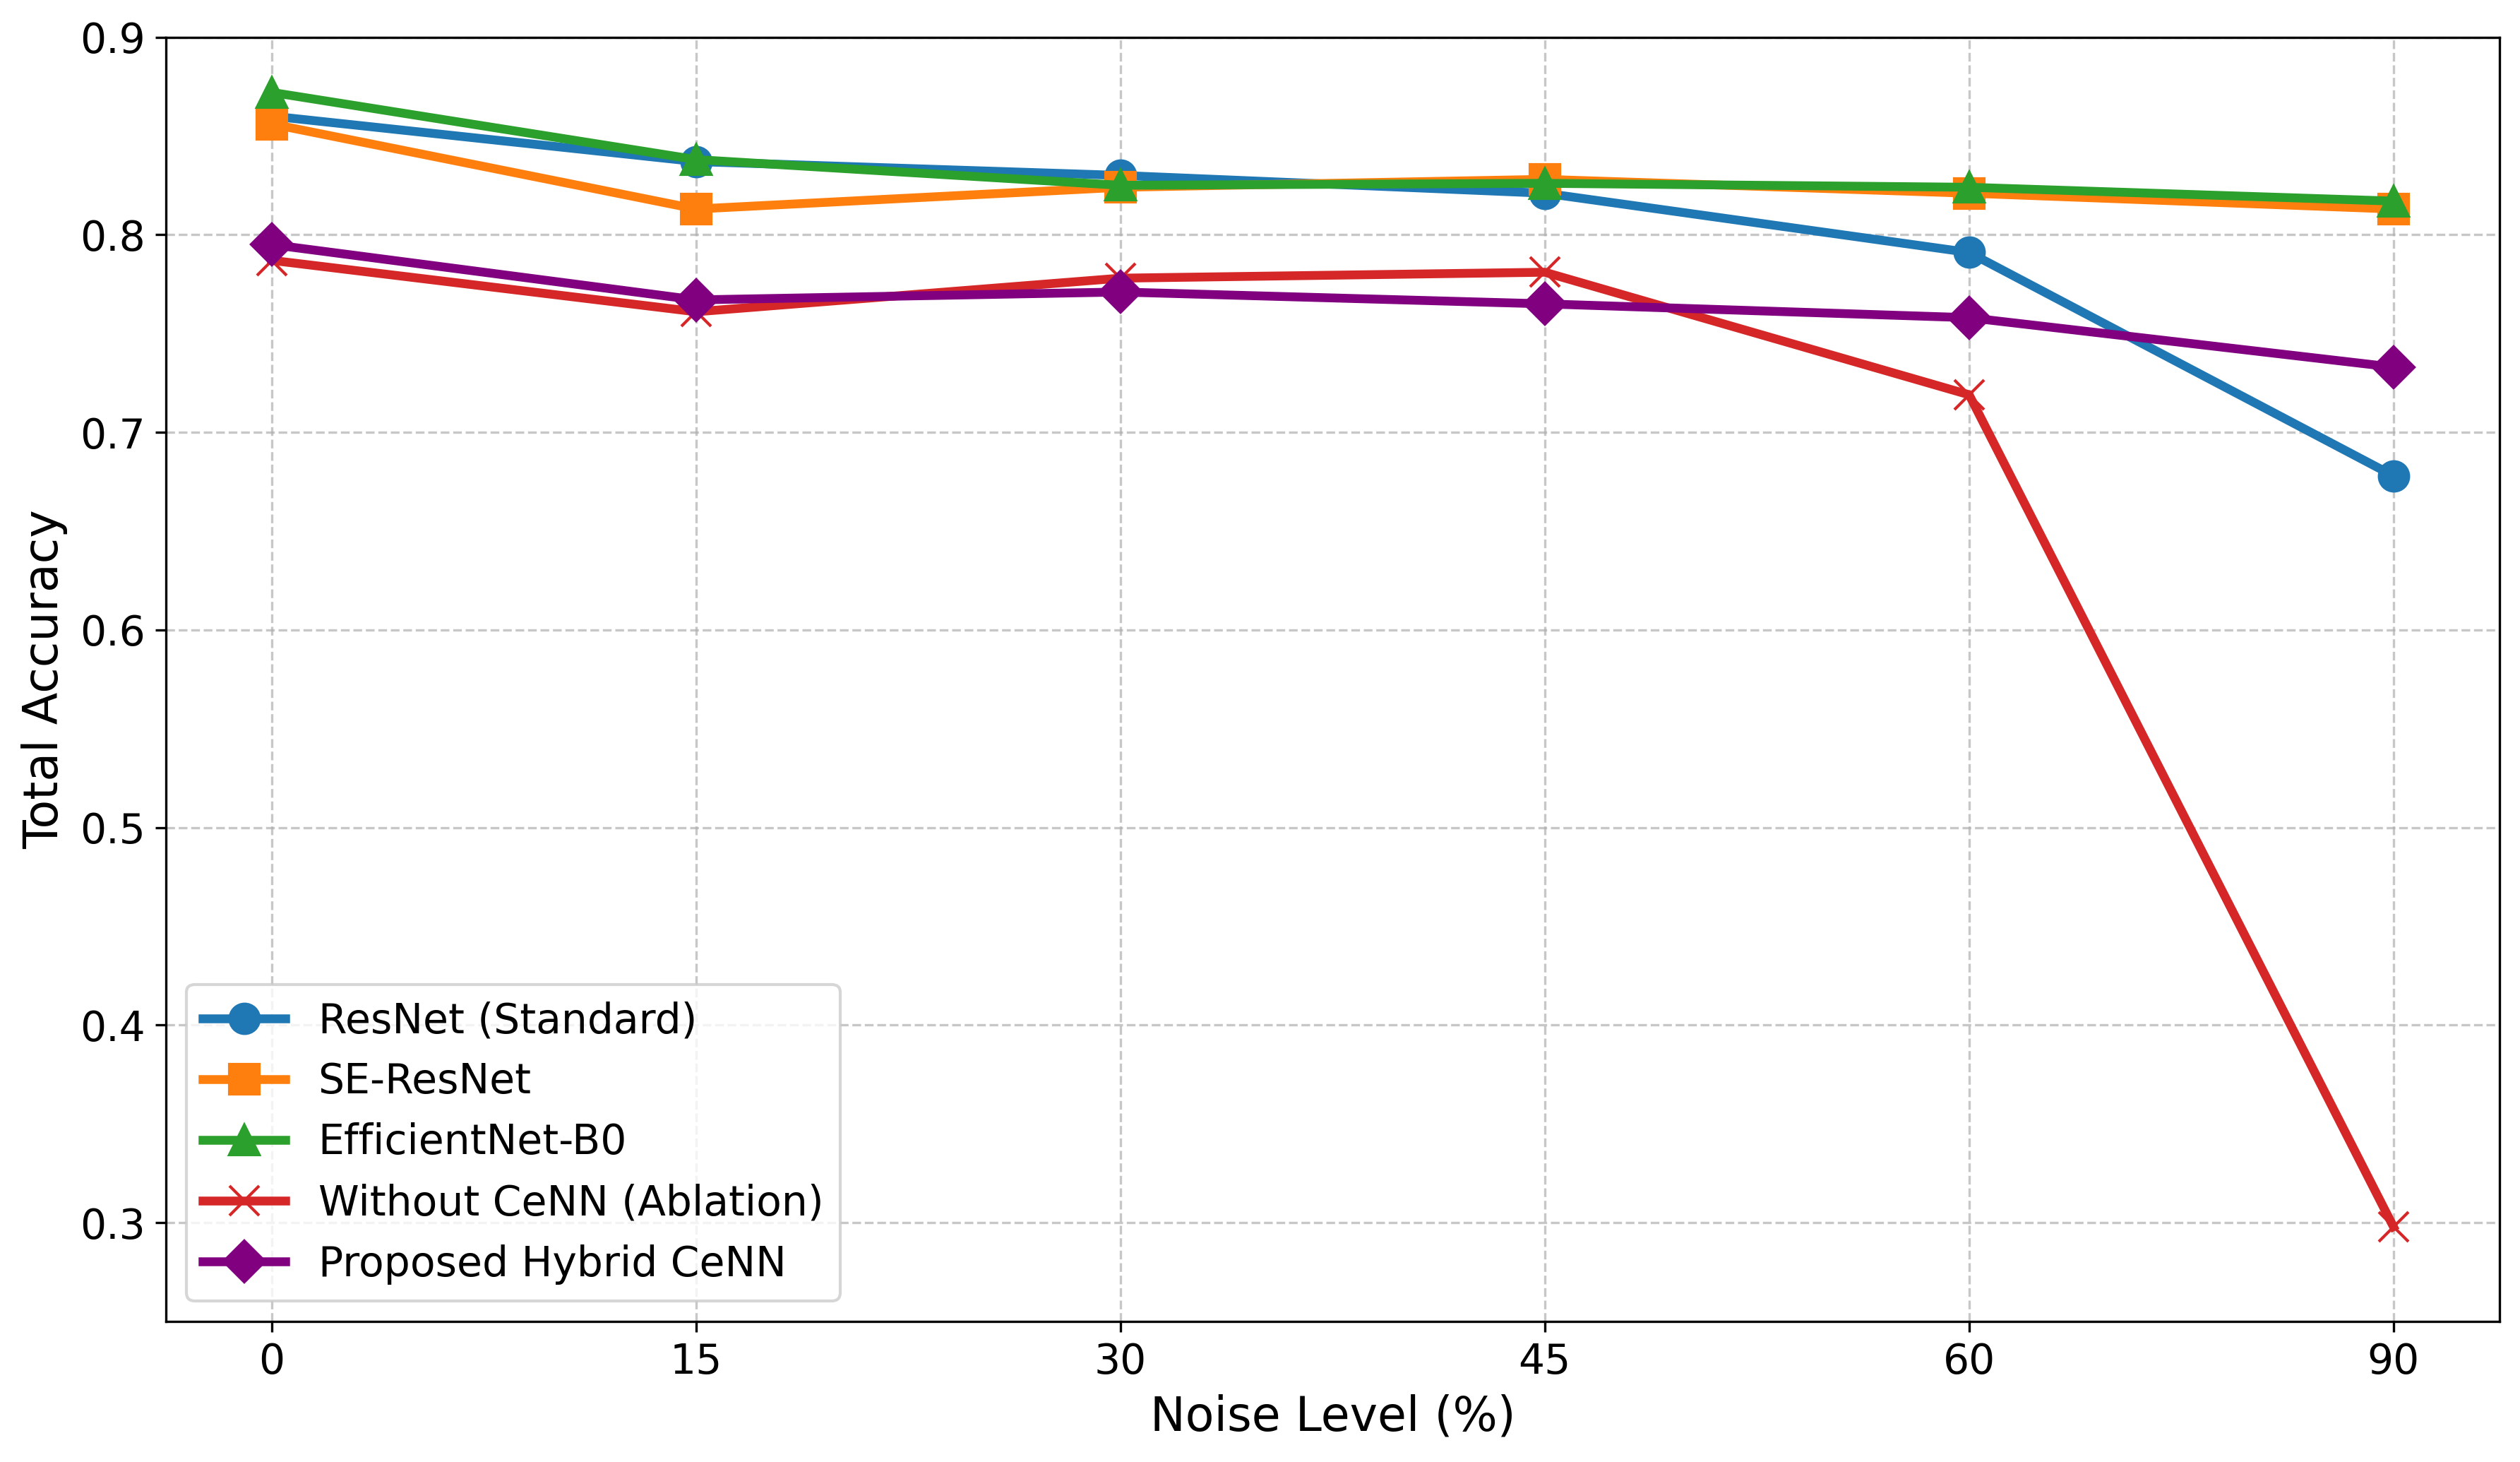
\includegraphics[width=\linewidth]{figs/conf_matr_noise/line_chart_zoomed.png}
	\captionof{figure}{Performance degradation of the evaluated architectures under increasing levels of Gaussian noise.}
	\label{fig:noise_line_chart}
\end{minipage}
\vspace{1em}

\section{Computational Efficiency and Inference Times}
A critical factor for the deployment of any medical Artificial Intelligence system is its computational footprint. Real-world clinical triage environments require systems that can process radiographs swiftly without necessitating prohibitive investments in top-tier server hardware. To evaluate this, we monitored both the training phase and the inference execution times.

\subsection{Training Phase}
The training of the multi-task architecture, including the computationally heavy continuous-time integration steps of the CeNN frontend, was conducted in a cloud environment using Kaggle Notebooks equipped with an NVIDIA Tesla P100 GPU (16GB VRAM). Thanks to the implementation of Virtual Batching (Gradient Accumulation), the memory footprint was kept manageable. The training process required approximately 15 to 20 minutes per epoch. Depending on the early stopping (patience) mechanism triggered by the validation loss, the total end-to-end training time ranged between 6 and 7 hours.

\subsection{Inference Phase and ASP Overhead}
To accurately simulate a deployment scenario in a resource-constrained local clinic, the inference benchmarks were executed on consumer-grade local hardware, specifically an NVIDIA GeForce GTX 1650 Super equipped with just 4GB of VRAM. 

First, we measured the inference time of the pure sub-symbolic neural network (CeNN + DenseNet + MTL Heads) on the entire dataset of 26,684 images.

As shown in Table \ref{tab:inference_raw}, despite the limited 4GB VRAM constraint, the pure neural pipeline is highly optimized. It processed the entire dataset in approximately 1,084 seconds, achieving a remarkable average inference time of 0.0406 seconds per image.

\begin{table}[htbp]
	\centering
	\caption{Inference benchmark for the raw Neural Network evaluated on the full dataset (26,684 images).}
	\label{tab:inference_raw}
	\begin{tabular*}{\linewidth}{@{\extracolsep{\fill}} >{\raggedright\arraybackslash}m{0.5\linewidth} r @{}}
		\toprule
		\textbf{Metric} & \textbf{Value} \\
		\midrule
		Total Inference Time & 1084.43 s \\
		Average Time per Image & 0.0406 s \\
		\bottomrule
	\end{tabular*}
\end{table}

Subsequently, we evaluated the computational overhead introduced by the Answer Set Programming (ASP) Semantic Validation Module. Because the ASP solver (clingo) relies on CPU-bound discrete logic grounding rather than GPU acceleration, it inherently introduces a bottleneck. We benchmarked the complete hybrid pipeline (Neural Network + ASP) on a random subset of 1,000 images.

\begin{table}[htbp]
	\centering
	\caption{Computational time breakdown for the complete Neuro-Symbolic pipeline (NN + ASP) evaluated on a 1,000-image subset.}
	\label{tab:inference_hybrid}
	\begin{tabular*}{\linewidth}{@{\extracolsep{\fill}} >{\raggedright\arraybackslash}m{0.5\linewidth} r @{}}
		\toprule
		\textbf{Component / Metric} & \textbf{Value} \\
		\midrule
		Neural Network (Average per Image) & 0.07059 s \\
		ASP Rules (Average per Image) & 0.01138 s \\
		\midrule
		\textbf{Total Pipeline Average per Image} & \textbf{0.08197 s} \\
		Total Time Spent (1,000 images) & 81.97 s \\
		\midrule
		Computational Load Distribution & NN: 86.12\% \textbar{} ASP: 13.88\% \\
		\bottomrule
	\end{tabular*}
\end{table}

Table \ref{tab:inference_hybrid} breaks down the computational load of the complete system. The average total processing time per image rises to 0.0819 seconds ($\sim$82 milliseconds). The Deep Learning perception engine accounts for 86.12\% of the execution time, while the ASP reasoning engine introduces a minimal overhead, taking just 0.0113 seconds ($\sim$11 milliseconds) per image and accounting for 13.88\% of the load. 

This result highlights the practical viability of the proposed architecture. Even with the introduction of an external logic solver to validate predictions, the complete hybrid system operates well under a tenth of a second per patient on entry-level hardware. This latency is largely imperceptible in an asynchronous radiological workflow, confirming that the significant gains in clinical safety (False Negative reduction) do not compromise the system's operational efficiency.

\subsection{Model Complexity and Hardware Footprint}
To fully address the computational footprint of the proposed architecture a comprehensive hardware profiling was conducted. The evaluation compares the proposed Hybrid CeNN model against standard baselines and an ablation model (identical architecture but lacking the CeNN frontend). The metrics extracted include the total parameter count, theoretical computational complexity (FLOPs), inference speed, throughput, and peak VRAM utilization.

\begin{table*}[htbp]
	\centering
	\caption{Hardware complexity, inference times, and resource consumption evaluated at a resolution of 512x512 with a batch size of 4.}
	\label{tab:hardware_metrics}
	\resizebox{\textwidth}{!}{%
		\begin{tabular}{lcccccc}
			\toprule
			\textbf{Model} & \textbf{Parameters (M)} & \textbf{Size (MB)} & \textbf{FLOPs (G)} & \textbf{Time / Batch (ms)} & \textbf{Throughput (img/s)} & \textbf{Peak VRAM (MB)} \\
			\midrule
			ResNet50 (Baseline) & 23.50 & 89.66 & 42.35 & 70.96 & 56.37 & 310.02 \\
			EfficientNet-B0 (Baseline) & 4.01 & 15.29 & 4.24 & 30.06 & 133.07 & 325.55 \\
			SE-ResNet50 (Baseline) & 26.03 & 99.31 & 42.35 & 79.01 & 50.63 & 427.36 \\
			\midrule
			Ablation: No CeNN & 18.48 & 70.50 & 33.32 & 78.86 & 50.72 & 451.39 \\
			\textbf{Proposed Hybrid CeNN} & \textbf{18.49} & \textbf{70.53} & \textbf{34.16} & \textbf{94.48} & \textbf{42.34} & \textbf{534.67} \\
			\bottomrule
		\end{tabular}%
	}
\end{table*}

As detailed in Table \ref{tab:hardware_metrics}, the integration of the CeNN frontend introduces a negligible structural overhead. Comparing the Ablation model to the Proposed Hybrid CeNN, the parameter count increases by merely 0.01 million (from 18.48 M to 18.49 M), and the model size expands by just 0.03 MB. While the continuous-time dynamics of the CeNN slightly elevate the FLOPs (34.16 G) and the peak VRAM usage (534.67 MB), the overall footprint remains significantly lower than standard deep models like SE-ResNet50 in terms of parameter volume.

Furthermore, an inference throughput of ~42 images per second demonstrates that the proposed architecture is highly suitable for real-time clinical screening. The minimal computational cost introduced by the bio-inspired frontend is heavily justified by the substantial gains in structural resilience and noise suppression demonstrated in the previous sections. Ultimately, these metrics confirm that the superior clinical safety achieved by the neuro-symbolic pipeline does not require prohibitive, server-tier hardware resources.

\section{Discussion and Limitations}
The results of our experimental evaluation underscore the potential of integrating bio-inspired pre-processing and symbolic reasoning into standard deep learning pipelines for medical imaging. By evaluating the system at various stages, we demonstrated that the hybrid architecture successfully mitigates two of the most critical flaws of purely statistical neural networks: vulnerability to input corruption and susceptibility to anatomically impossible hallucinations.

\subsection{The Clinical Trade-off: Statistical Thresholding vs. Neuro-Symbolic Rescue}
A central finding of this study is the confirmation that global accuracy is an inadequate metric for evaluating medical triage systems. True clinical utility often requires deliberately sacrificing statistical precision to maximize Sensitivity (Recall). By formally encoding the premise that a False Negative is exponentially more dangerous than a False Positive, our system successfully aligns the AI's behavior much closer to human clinical protocols.

A critical methodological evaluation arises when comparing the purely statistical threshold optimization (reducing the global decision boundary to 0.4) against the application of the ASP Semantic Validation Module operating on the default 0.5 boundary. Lowering the global classification threshold to 0.4, as explored during the Test-Time Augmentation phase, is a "brute-force" statistical approach. It successfully forces the network to become more sensitive, lowering False Negatives to 1,499. However, this method is anatomically blind; it statistically accepts lower-probability predictions regardless of their spatial location or geometric plausibility, inadvertently accepting artifacts and confounding structures.

In contrast, the Neuro-Symbolic ASP integration represents an "intelligent rescue" paradigm. By maintaining the baseline neural network threshold at 0.5 (which inherently produced 2,325 False Negatives), the ASP module acts selectively. It rescued sub-threshold opacities only if they exhibited biologically plausible characteristics. For instance, the "Organic" configuration specifically rescued sub-threshold opacities only if they exhibited biologically plausible aspect ratios and sizes, successfully dropping the False Negatives down to 1,221. 

Consequently, the ASP logic outperforms the best purely statistical threshold strategy (1,221 vs. 1,499 False Negatives). This proves that embedding explicit medical knowledge via logic programming is significantly more effective and clinically safer than blindly adjusting statistical confidence bounds, effectively shifting the paradigm from purely data-driven classification to safety-first, logic-bounded medical prediction.

\subsection{Computational Overhead}
Despite its robustness, the proposed architecture introduces a noticeable computational overhead compared to a standalone Convolutional Neural Network. The continuous-time dynamic approximation required by the CeNN frontend necessitates multiple unrolled integration steps, increasing the memory footprint and the latency during the forward pass. 

Furthermore, the Semantic Validation Module relies on clingo, an external ASP solver. While grounding and solving the relatively small Knowledge Base for a single image takes only a fraction of a second, this discrete logic step breaks the end-to-end differentiability of the pipeline and adds a computational bottleneck. However, as demonstrated in our inference benchmarks, the system still operates well under a tenth of a second per patient even on consumer-grade hardware. Given that radiographic screening is typically an asynchronous, batch-processed task rather than a strict real-time video processing requirement, this latency is highly acceptable in exchange for diagnostic safety.

\subsection{Generalization and Rule Engineering}
A notable limitation of the current Neuro-Symbolic implementation is the reliance on hand-crafted, domain-specific logic rules. The geometric and spatial constraints (such as the safe zones or the organic aspect ratios) were explicitly engineered for frontal Chest X-rays (CXR) targeting pneumonia. Consequently, these rules will not generalize out-of-the-box to lateral CXR views, pediatric radiographs, or different pathologies without expert medical re-calibration.

Additionally, while the DenseNet-121 backbone leverages transfer learning to mitigate domain gaps, the model's overall statistical perception remains bounded by the diversity of the RSNA dataset. Future iterations of this work must evaluate the system's robustness against dataset shift, particularly when processing images acquired from different radiological equipment or demographic distributions.

\subsection{Evaluating a BD-CeNN Autoencoder Pre-processing Hypothesis}

During the development of the proposed architecture, we thoroughly investigated the hypothesis of incorporating an explicit Autoencoder as a pre-processing stage for direct image reconstruction and denoising. Specifically, this module was designed as a Bidirectional Cellular Neural Network (BD-CeNN) Autoencoder, ensuring that the entire pipeline remained grounded in the core CeNN paradigm. The theoretical premise was to aggressively filter Gaussian noise before passing the reconstructed image to the DenseNet-121 backbone.

However, empirical validation revealed critical limitations in this approach for the specific domain of pneumonia detection. While the BD-CeNN autoencoder successfully suppressed artificial noise, it inadvertently induced an "over-smoothing" effect on the reconstructed images. Pneumonia opacities typically present as subtle, diffuse textures rather than solid objects with sharp, distinct boundaries. The autoencoder smoothed out these critical pathological semantics alongside the noise, significantly degrading the model's discriminative power.

As illustrated in Figure \ref{fig:autoencoder_noise}, under extreme noise conditions (90\% variance), the accuracy of the autoencoder-based model collapsed to 62.6\%, accompanied by a severe spike in False Positives (1,797 cases). In contrast, our proposed architecture, which utilizes the CeNN solely as a dynamic feature extractor rather than an image reconstructor, maintained a much more robust performance under the same conditions.

%\noindent
%\begin{minipage}{\linewidth}
%	\centering
%	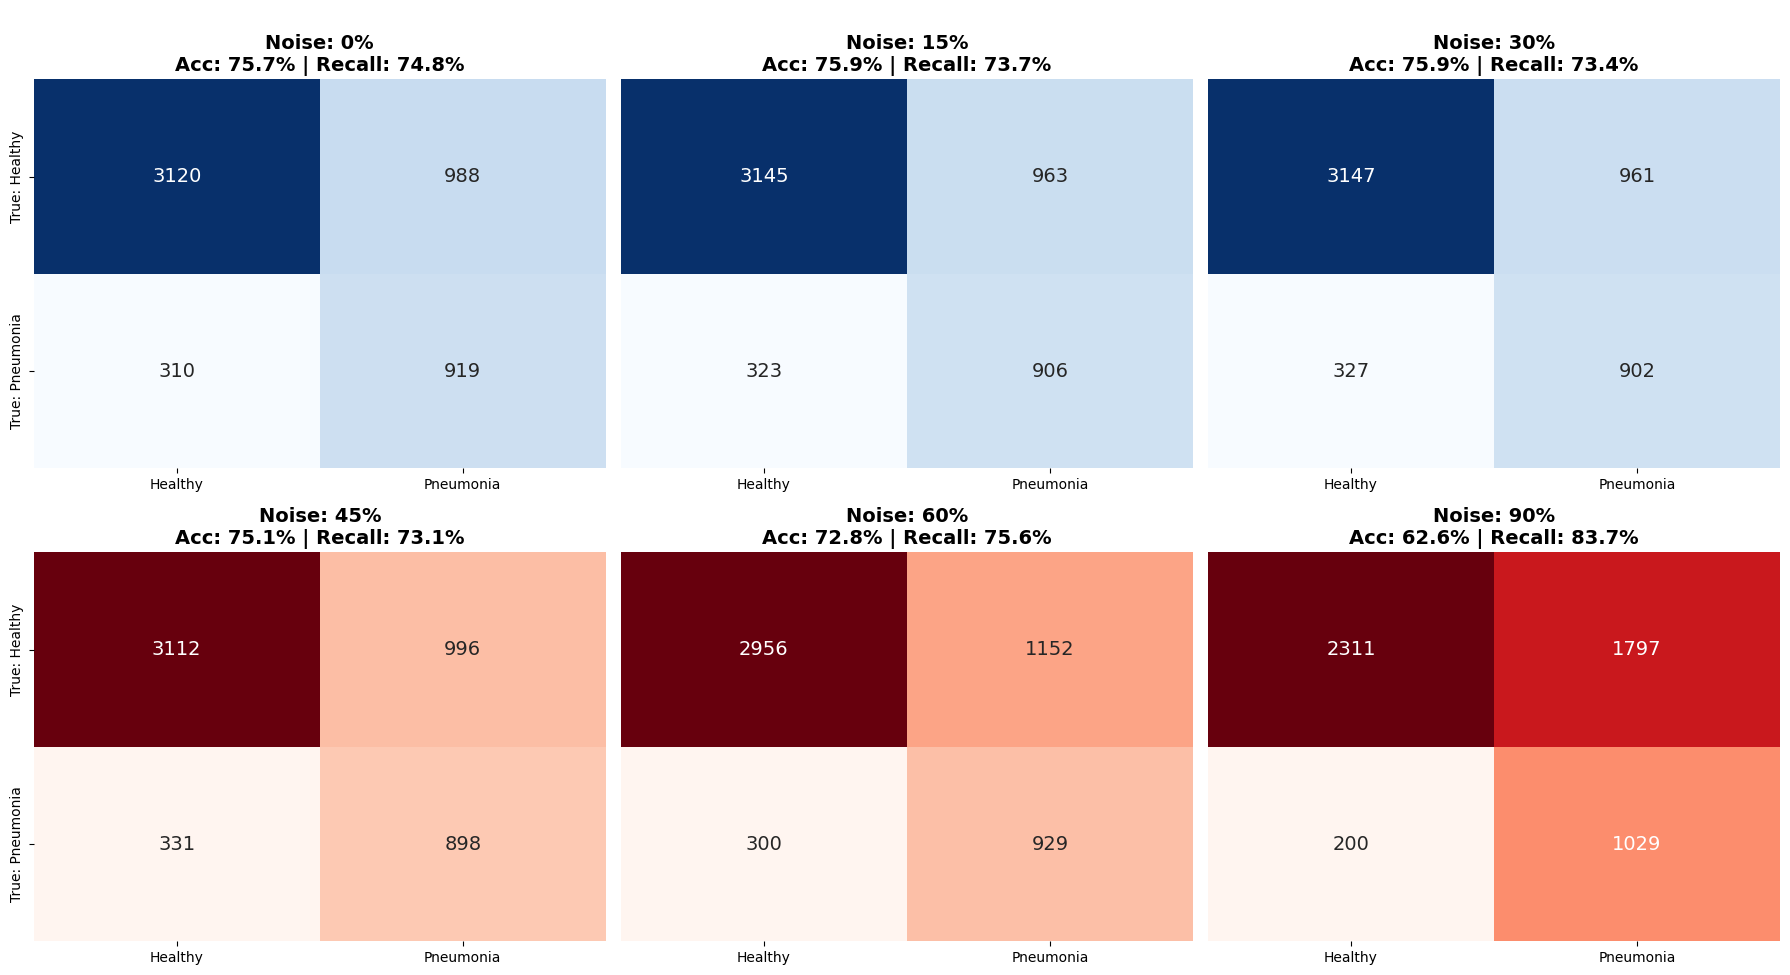
\includegraphics[width=\textwidth]{figs/autoencoder_noise.png}
%	\captionof{figure}{Confusion matrices demonstrating the performance degradation of the BD-CeNN Autoencoder hypothesis under varying levels of Gaussian noise. Note the severe drop in Accuracy and the spike in False Positives at the 90\% noise level due to image over-smoothing.}
%	\label{fig:autoencoder_noise}
%\end{minipage}
%\vspace{1em}

\begin{figure*}[htbp]
	\centering
	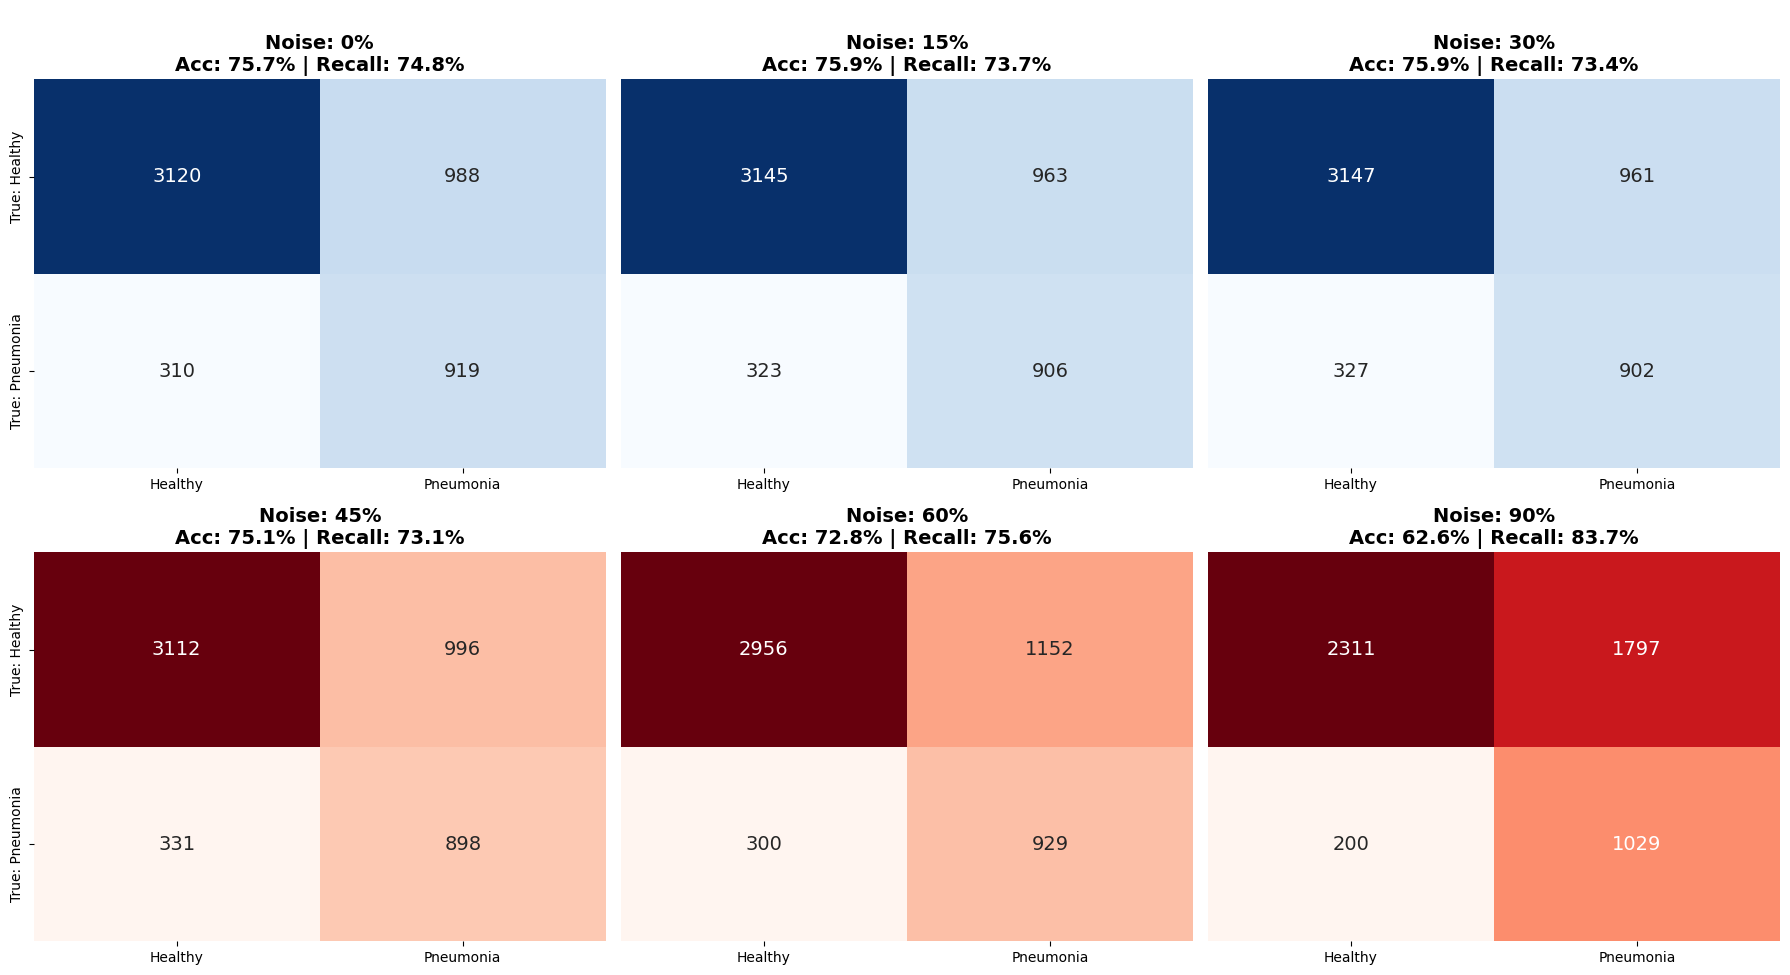
\includegraphics[width=0.9\textwidth]{figs/autoencoder_noise.png}
	\caption{Confusion matrices demonstrating the performance degradation of the BD-CeNN Autoencoder hypothesis under varying levels of Gaussian noise. Note the severe drop in Accuracy and the spike in False Positives at the 90\% noise level due to image over-smoothing.}
	\label{fig:autoencoder_noise}
\end{figure*}

Furthermore, the inclusion of the generative autoencoder module drastically increased the computational burden, extending the training phase to over 10 hours, without yielding proportional clinical benefits. 

Consequently, we concluded that our original hybrid approach is structurally superior for this specific medical task. Nevertheless, we remain open to future developments and alternative implementations that might successfully integrate generative pre-processing steps in this domain, though exploring these possibilities remains outside the scope of the current work.

\section{Conclusion and Future Work}
In this paper, we presented a novel hybrid neuro-symbolic architecture for robust image recognition and localization, specifically tailored for the challenging domain of medical radiography. By addressing the inherent vulnerabilities of standard convolutional networks, namely, their susceptibility to signal noise and their inability to comprehend spatial and anatomical context, we developed a pipeline that prioritizes clinical safety over raw statistical metrics.

Our experimental evaluations validated the core hypotheses of this work. First, the comparative benchmarking and ablation study confirmed that the integration of a bio-inspired Cellular Neural Network (CeNN) frontend acts as a highly effective continuous-time stabilizer. While highly parameterized, single-task architectures like ResNet and the isolated DenseNet baseline structurally collapsed under extreme Gaussian noise (dropping to 67.8\% and 29.8\% accuracy, respectively), the proposed CeNN-augmented model exhibited exceptional structural resilience. Despite the heavier optimization burden of the Multi-Task Learning formulation, our hybrid architecture maintained a highly stable degradation curve, losing only 6.2\% accuracy across the entire noise spectrum and proving its strengths in maintaining reliable feature extraction in highly corrupted environments.

Second, the implementation of the Answer Set Programming (ASP) Semantic Validation Module demonstrated that sub-symbolic perception can be vastly improved by explicit logical reasoning. By enforcing geometric and biological constraints on sub-threshold predictions, the neuro-symbolic logic successfully reduced the False Negatives, significantly outperforming the best purely statistical approach.

Looking ahead, several promising avenues for future research emerge to address the current limitations of the system.

\subsection{Expert-Driven Rule Engineering}
A primary limitation of the current Neuro-Symbolic implementation is that the Knowledge Base was manually engineered by a non-medical expert, leveraging the Gemini AI chatbot for the brainstorming and formalization of basic geometric rules. While this proved highly effective for a proof-of-concept, an active collaboration with certified radiologists is essential. Medical professionals could define much more precise, nuanced, and clinically accurate ASP constraints, elevating the system from a computational experiment to a deployable diagnostic tool. Alternatively, exploring Inductive Logic Programming (ILP) to automatically extract and formalize medical constraints directly from annotated datasets or radiological reports would make the semantic validation module highly scalable.

\subsection{Dataset Diversity and Scale}
The model's overall statistical perception currently relies on the RSNA Pneumonia dataset. While valuable, this dataset presents a relatively low number of positive pathological images and lacks broad demographic and equipment diversity. Evaluating the architecture's generalization capabilities across multi-center datasets is a crucial next step to ensure robustness against dataset shifts.

\subsection{Computational Scaling}
The training phase of this hybrid architecture proved to be highly computationally intensive, requiring 6 to 7 hours on cloud hardware (NVIDIA Tesla P100) due to the continuous-time dynamics of the CeNN and the high-resolution inputs. Consequently, the network size, the number of epochs, and the image resolution (capped at 512x512) were constrained by time and memory limits. With access to more advanced hardware clusters, future iterations could scale up the pipeline to process images at their native 1024x1024 resolution, utilize deeper backbone architectures, and extend the training regime without relying on aggressive early stopping.

Despite these limitations, the proposed architecture successfully bridges the gap between robust low-level signal processing and high-level medical reasoning, paving the way for safer and more transparent AI screening tools in critical clinical triage environments.

\clearpage

\section*{Code Availability}
To ensure full transparency and reproducibility of the experiments presented in this study, the complete and modular Python codebase has been made publicly available. The repository includes the neural network architectures, the multi-task training pipeline, the hardware profiling scripts, and the declarative Answer Set Programming (ASP) rules (.lp files) used for the neuro-symbolic semantic validation. 

The source code, along with detailed setup instructions, can be accessed on GitHub at: \url{https://github.com/N1ck219/NeuroSymbolic-Pneumonia-Detection}

Due to file size constraints, the pre-trained model weights (.pth files) are hosted externally on a dedicated cloud storage drive. The download links and instructions for replicating the inference and noise robustness tests are thoroughly documented within the repository's \texttt{README.md} file.

\section*{Declaration of Generative AI and AI-assisted technologies}

During the preparation of this work, the author used Google Gemini to assist in various phases of the research and manuscript drafting. Specifically, the AI was utilized to gain an initial theoretical understanding of Cellular Neural Networks (CeNN) and for preliminary brainstorming prior to the software development phase. During coding, Gemini assisted in debugging and facilitated the implementation of specific architectural components, such as the Convolutional Block Attention Module (CBAM). Furthermore, generative AI tools were employed to design the schematic figures representing the proposed network architecture and the CeNN dynamics. 

Finally, during the writing process, the author drafted the foundational structure of the manuscript in their native language, and Gemini was used to translate the text and refine the academic tone and phrasing. After using these tools, the author thoroughly reviewed and edited all contents as needed, and takes full and sole responsibility for the accuracy, originality, and integrity of the final publication.


\clearpage 

\bibliographystyle{elsarticle-num} 
\bibliography{cas-refs}

\clearpage 
	
\appendix
\section{Detailed Noise Robustness Results}
\label{sec:appendix_matrices}

\begin{strip}
This appendix provides the comprehensive evaluation metrics and the detailed confusion matrices for all the architectures tested during the noise robustness benchmarking discussed in Section \ref{sec:comparative_analysis}.

	\vspace{1em}
	\centering
	\captionof{table}{Model Accuracy across increasing levels of Gaussian Noise. \textit{Note: These benchmarks were conducted on a representative subset of the test data to accommodate the computational overhead of multi-level noise injection; baseline values (0\%) may therefore differ slightly from full-dataset results in Table \ref{tab:master_results}.}}
	\label{tab:noise_accuracy}
	\resizebox{\textwidth}{!}{%
		\begin{tabular}{lcccccc}
			\hline
			\textbf{Model} & \textbf{0\%} & \textbf{15\%} & \textbf{30\%} & \textbf{45\%} & \textbf{60\%} & \textbf{90\%} \\
			\hline
			ResNet50 & 86.0\% & 83.7\% & 83.0\% & 82.1\% & 79.1\% & 67.8\% \\
			SE-ResNet50 & 85.6\% & 81.3\% & 82.4\% & 82.8\% & 82.1\% & 81.3\% \\
			EfficientNet-B0 & 87.2\% & 83.8\% & 82.5\% & 82.6\% & 82.4\% & 81.7\% \\
			Without CeNN (Ablation) & 78.7\% & 76.1\% & 77.8\% & 78.1\% & 71.9\% & 29.8\% \\
			\textbf{Proposed CeNN Hybrid} & \textbf{79.5\%} & \textbf{76.7\%} & \textbf{77.1\%} & \textbf{76.5\%} & \textbf{75.8\%} & \textbf{73.3\%} \\
			\hline
		\end{tabular}%
	}


\end{strip}

\clearpage

% --- BLOCCO 1: Prime due immagini ---
\begin{figure*}[htbp]
	\centering
	\begin{subfigure}{\linewidth}
		\centering
		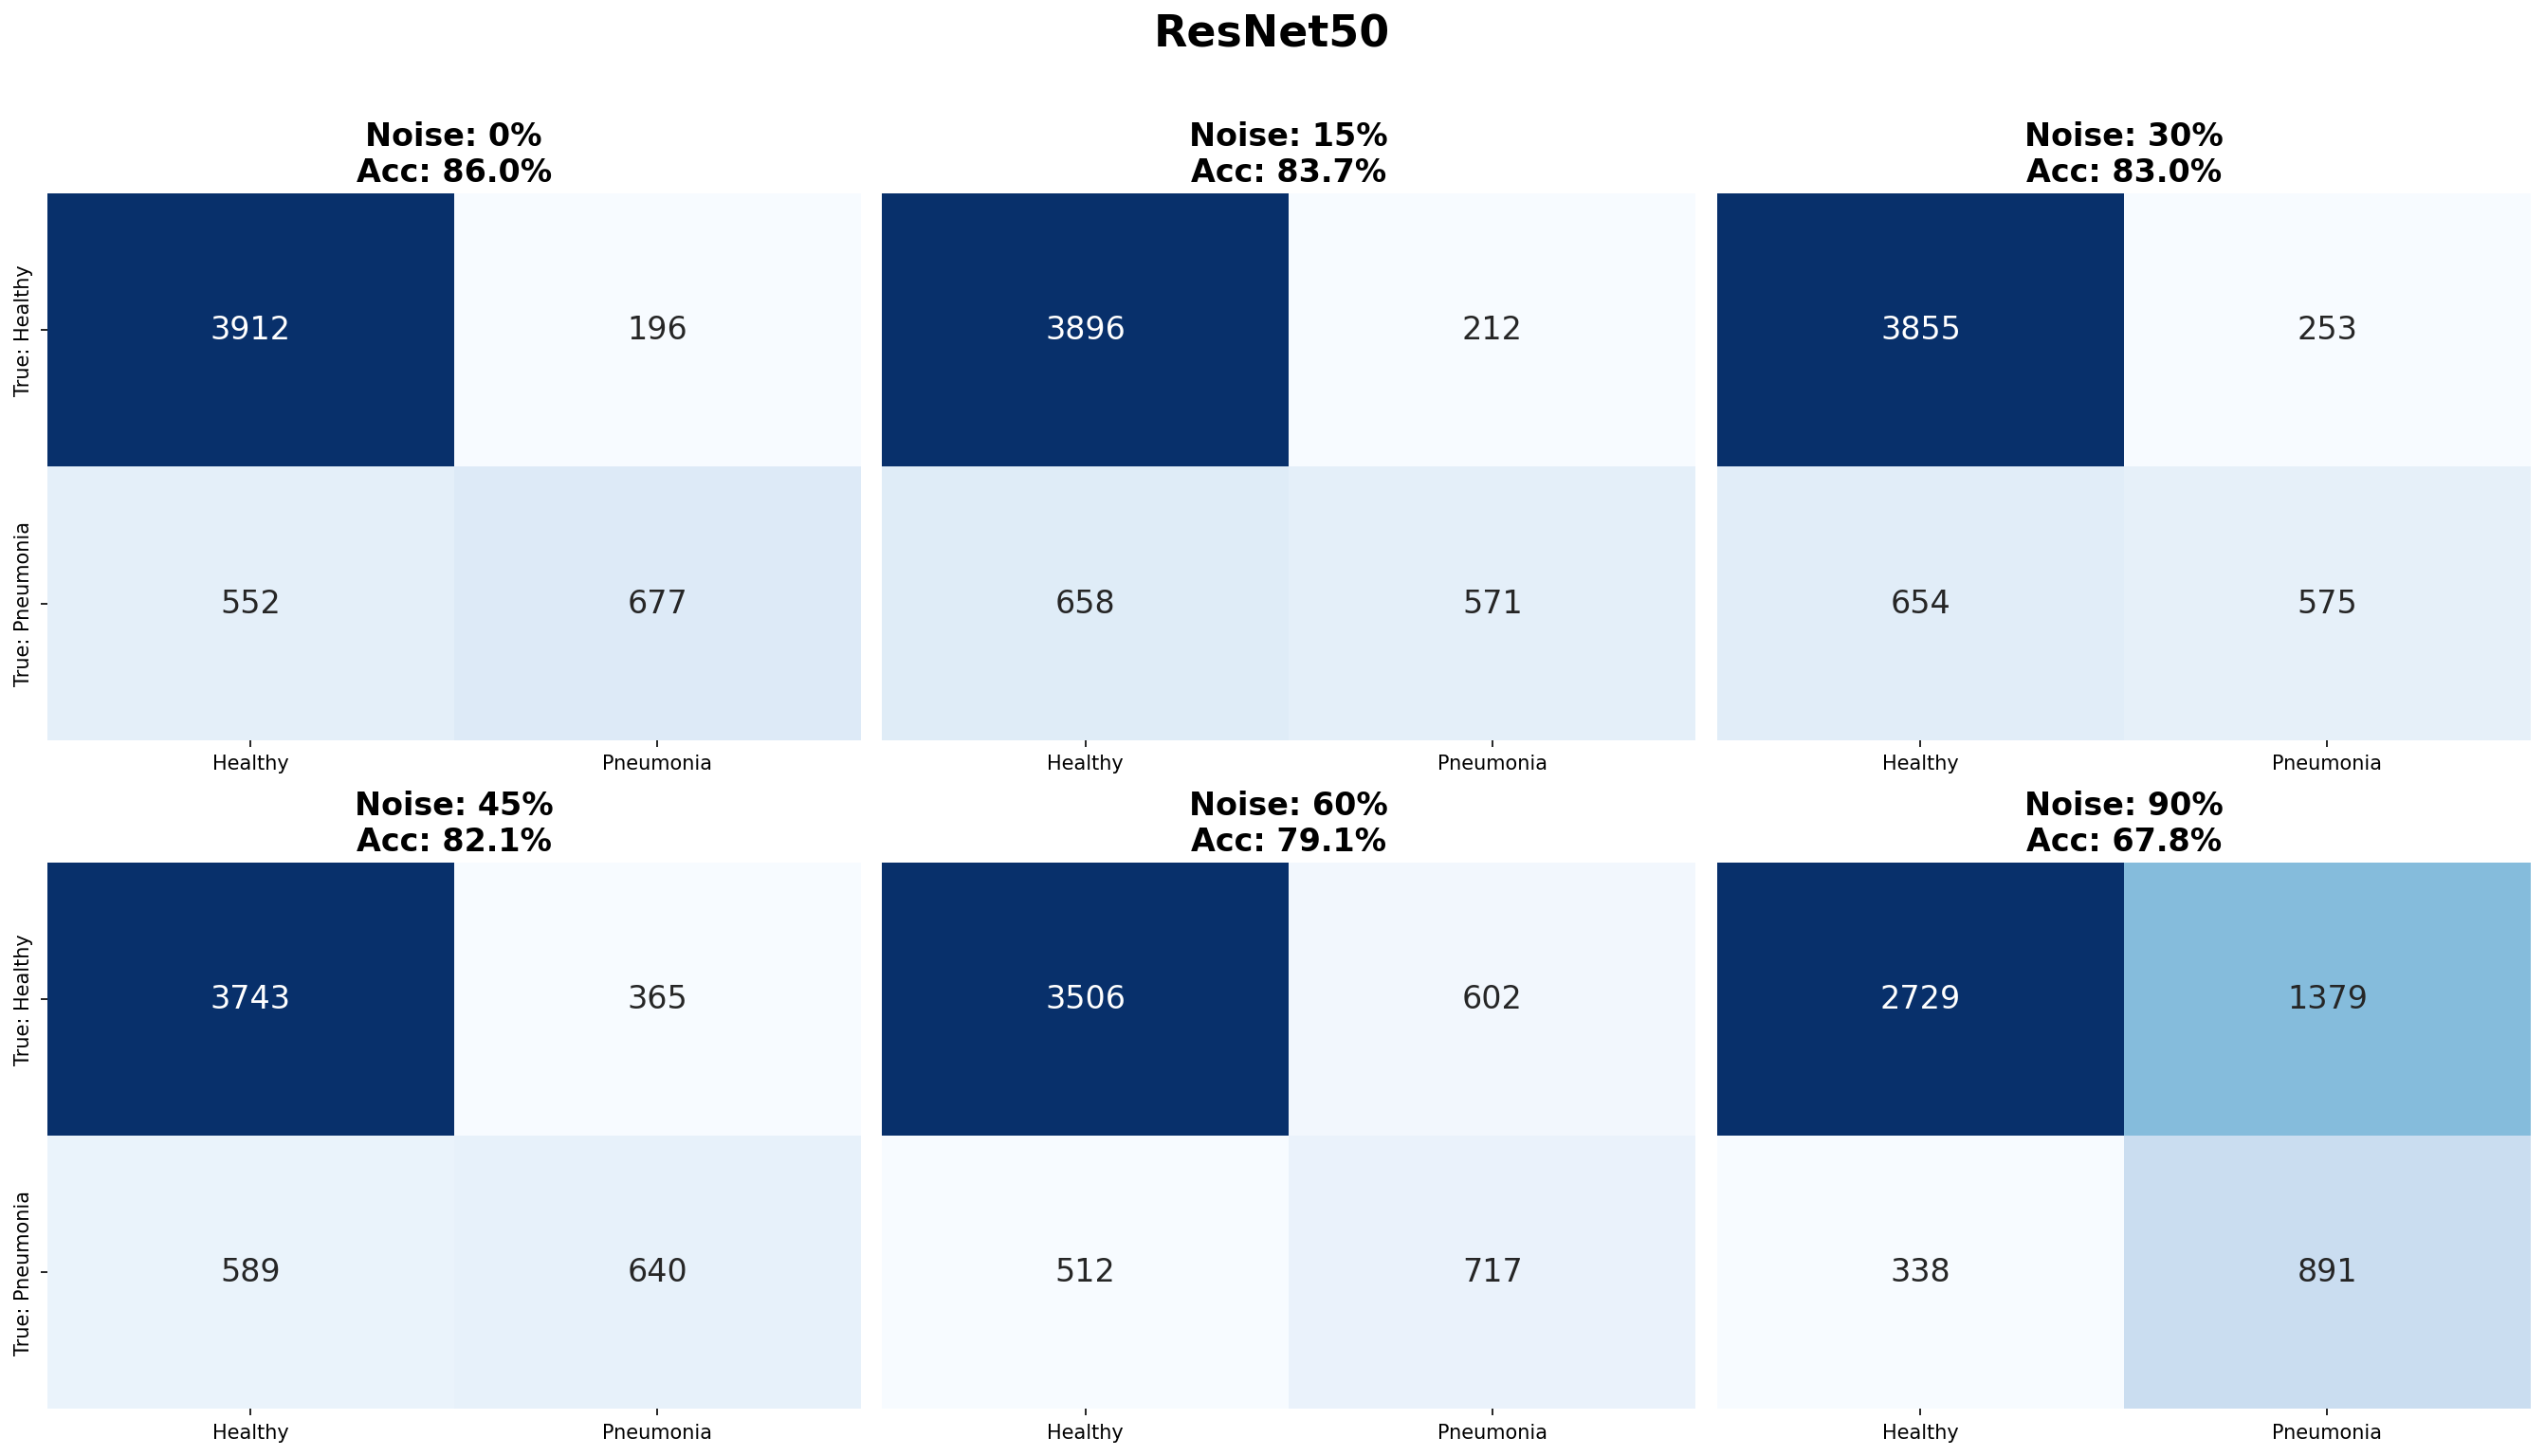
\includegraphics[width=0.85\linewidth]{figs/conf_matr_noise/ResNet50_CM.png}
		\caption{ResNet (Standard)}
		\label{fig:sub_resnet}
	\end{subfigure}
	\vspace{1em} % Aumentato leggermente lo spazio tra le immagini
	
	\begin{subfigure}{\linewidth}
		\centering
		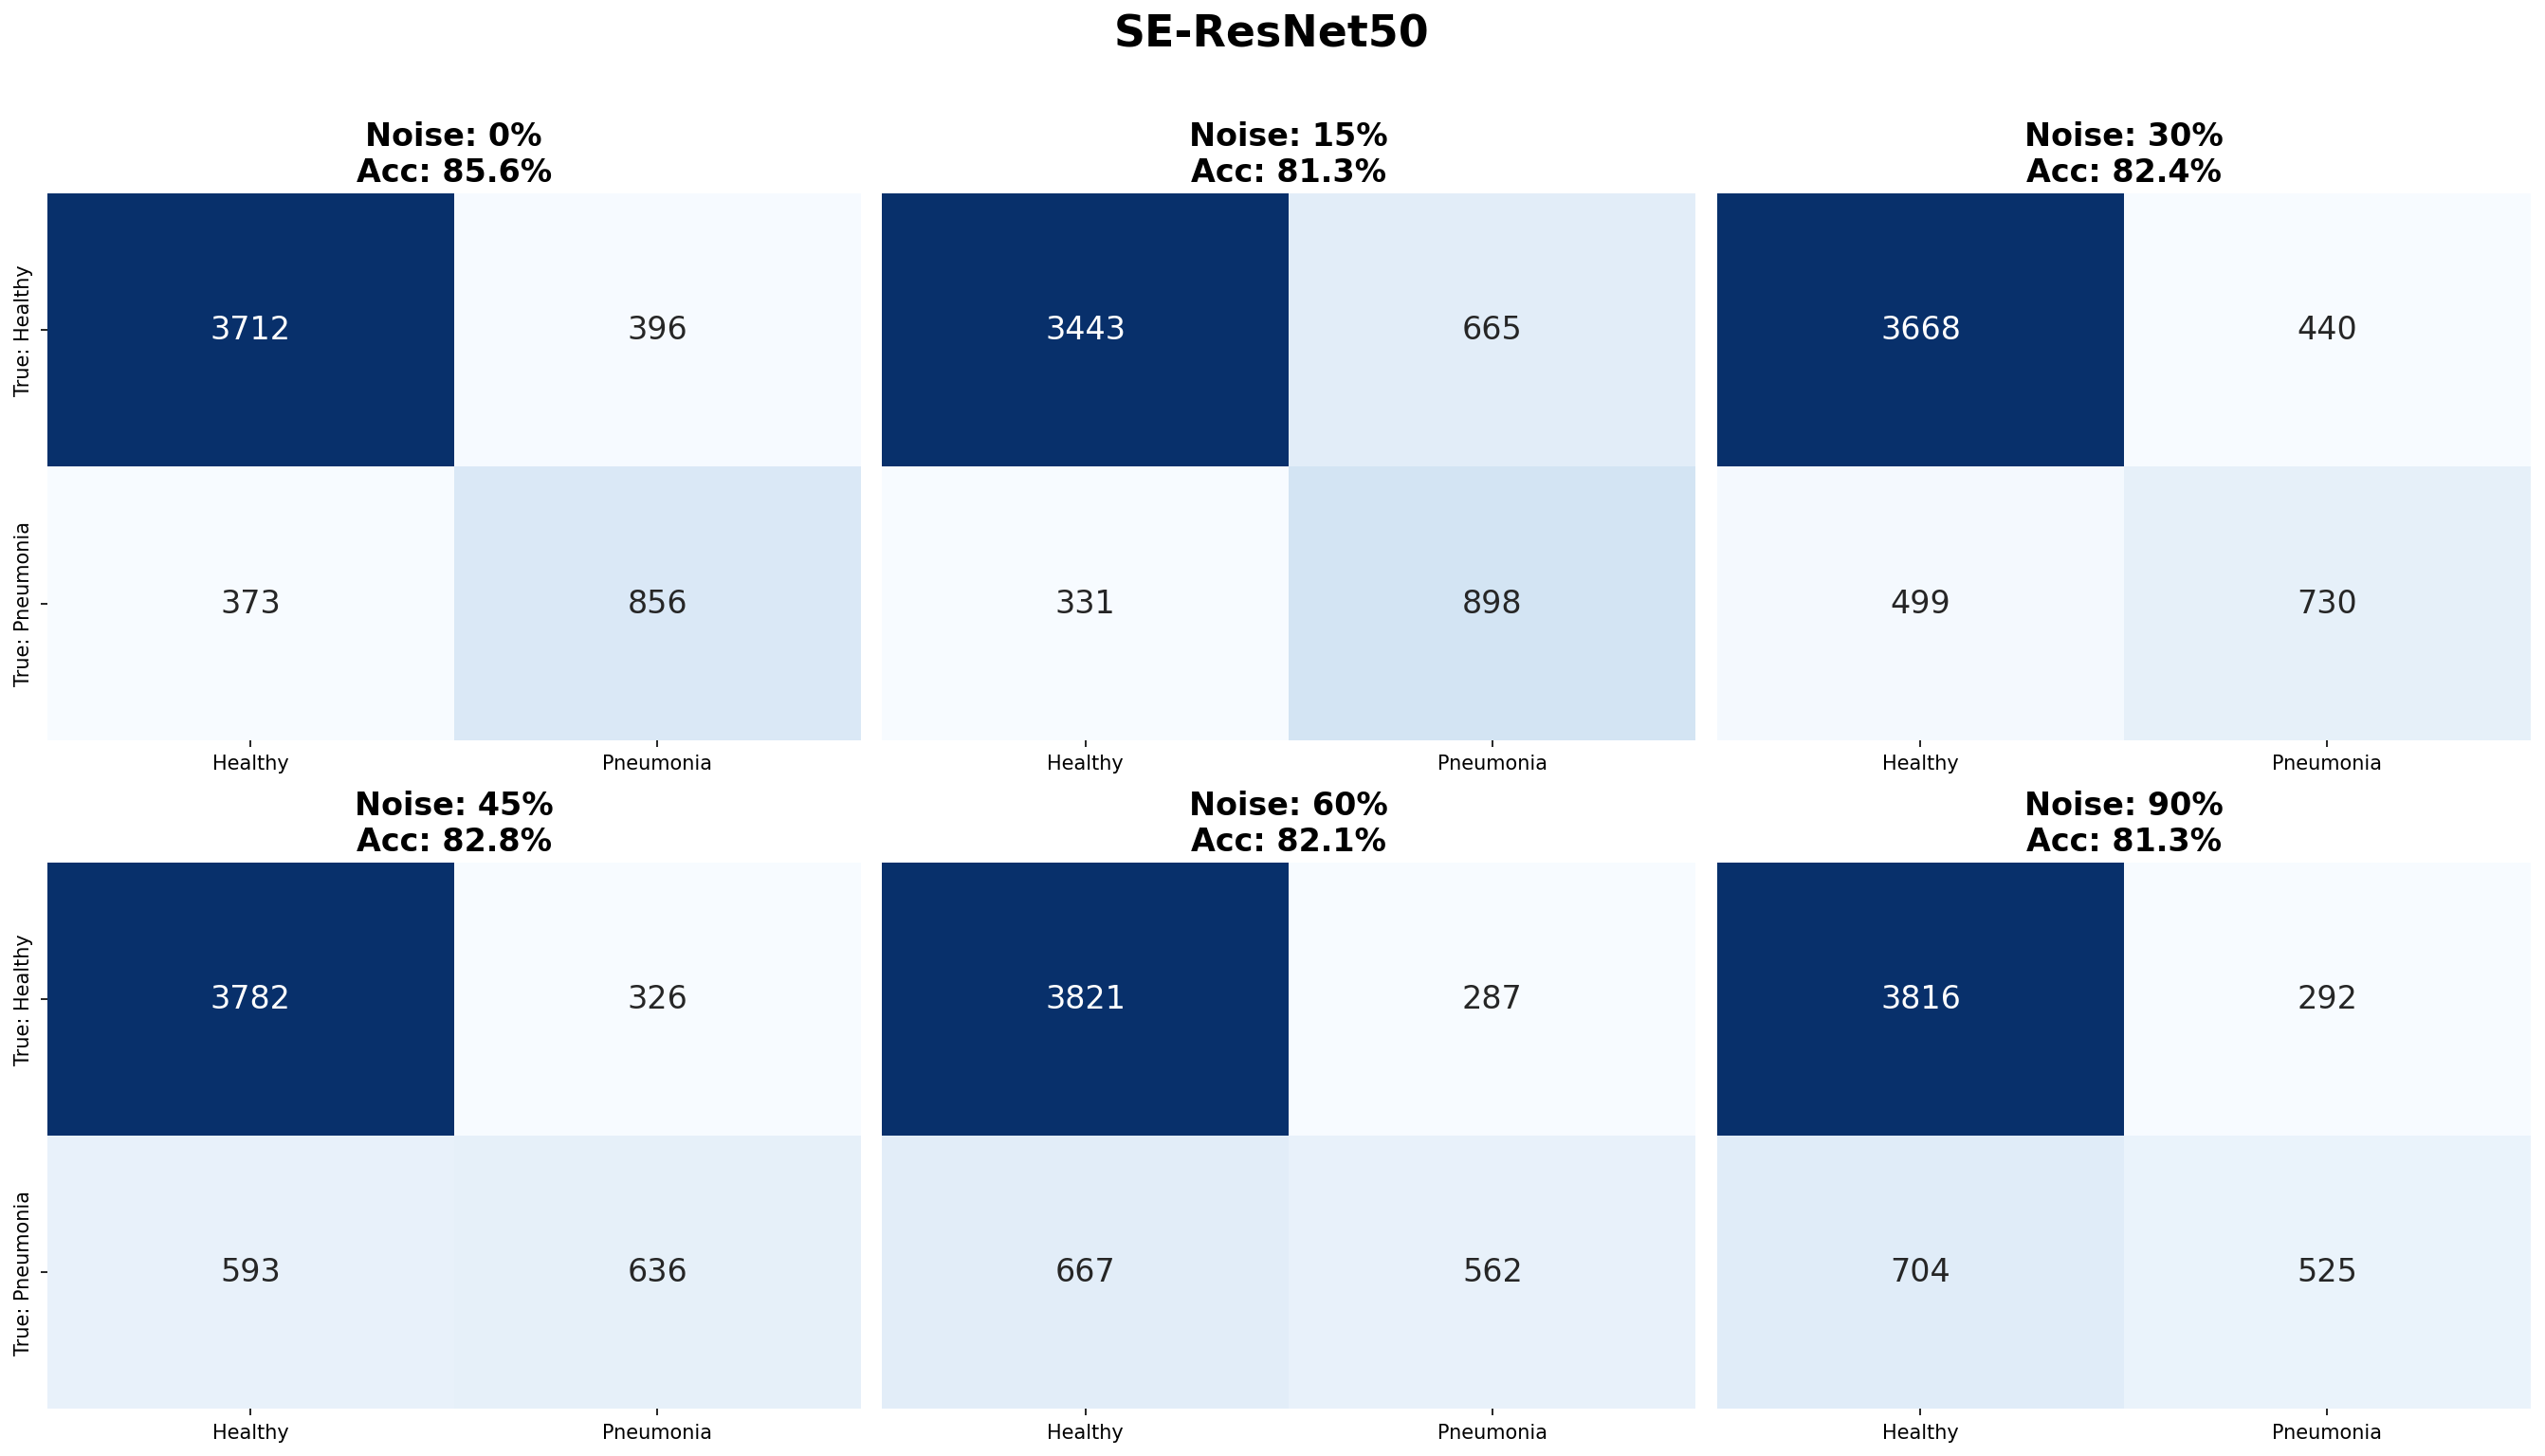
\includegraphics[width=0.85\linewidth]{figs/conf_matr_noise/SE-ResNet50_CM.png}
		\caption{SE-ResNet}
		\label{fig:sub_seresnet}
	\end{subfigure}
	
	\caption{Detailed Confusion Matrices across different architectures (Part 1). Performance is monitored from $0\%$ to $90\%$ Gaussian noise variance.}
	\label{fig:noise_comparison_p1}
\end{figure*}

% --- BLOCCO 2: Terza e Quarta immagine ---
\begin{figure*}[htbp]
	\ContinuedFloat % Continua la numerazione della Figura precedente
	\centering
	\begin{subfigure}{\linewidth}
		\centering
		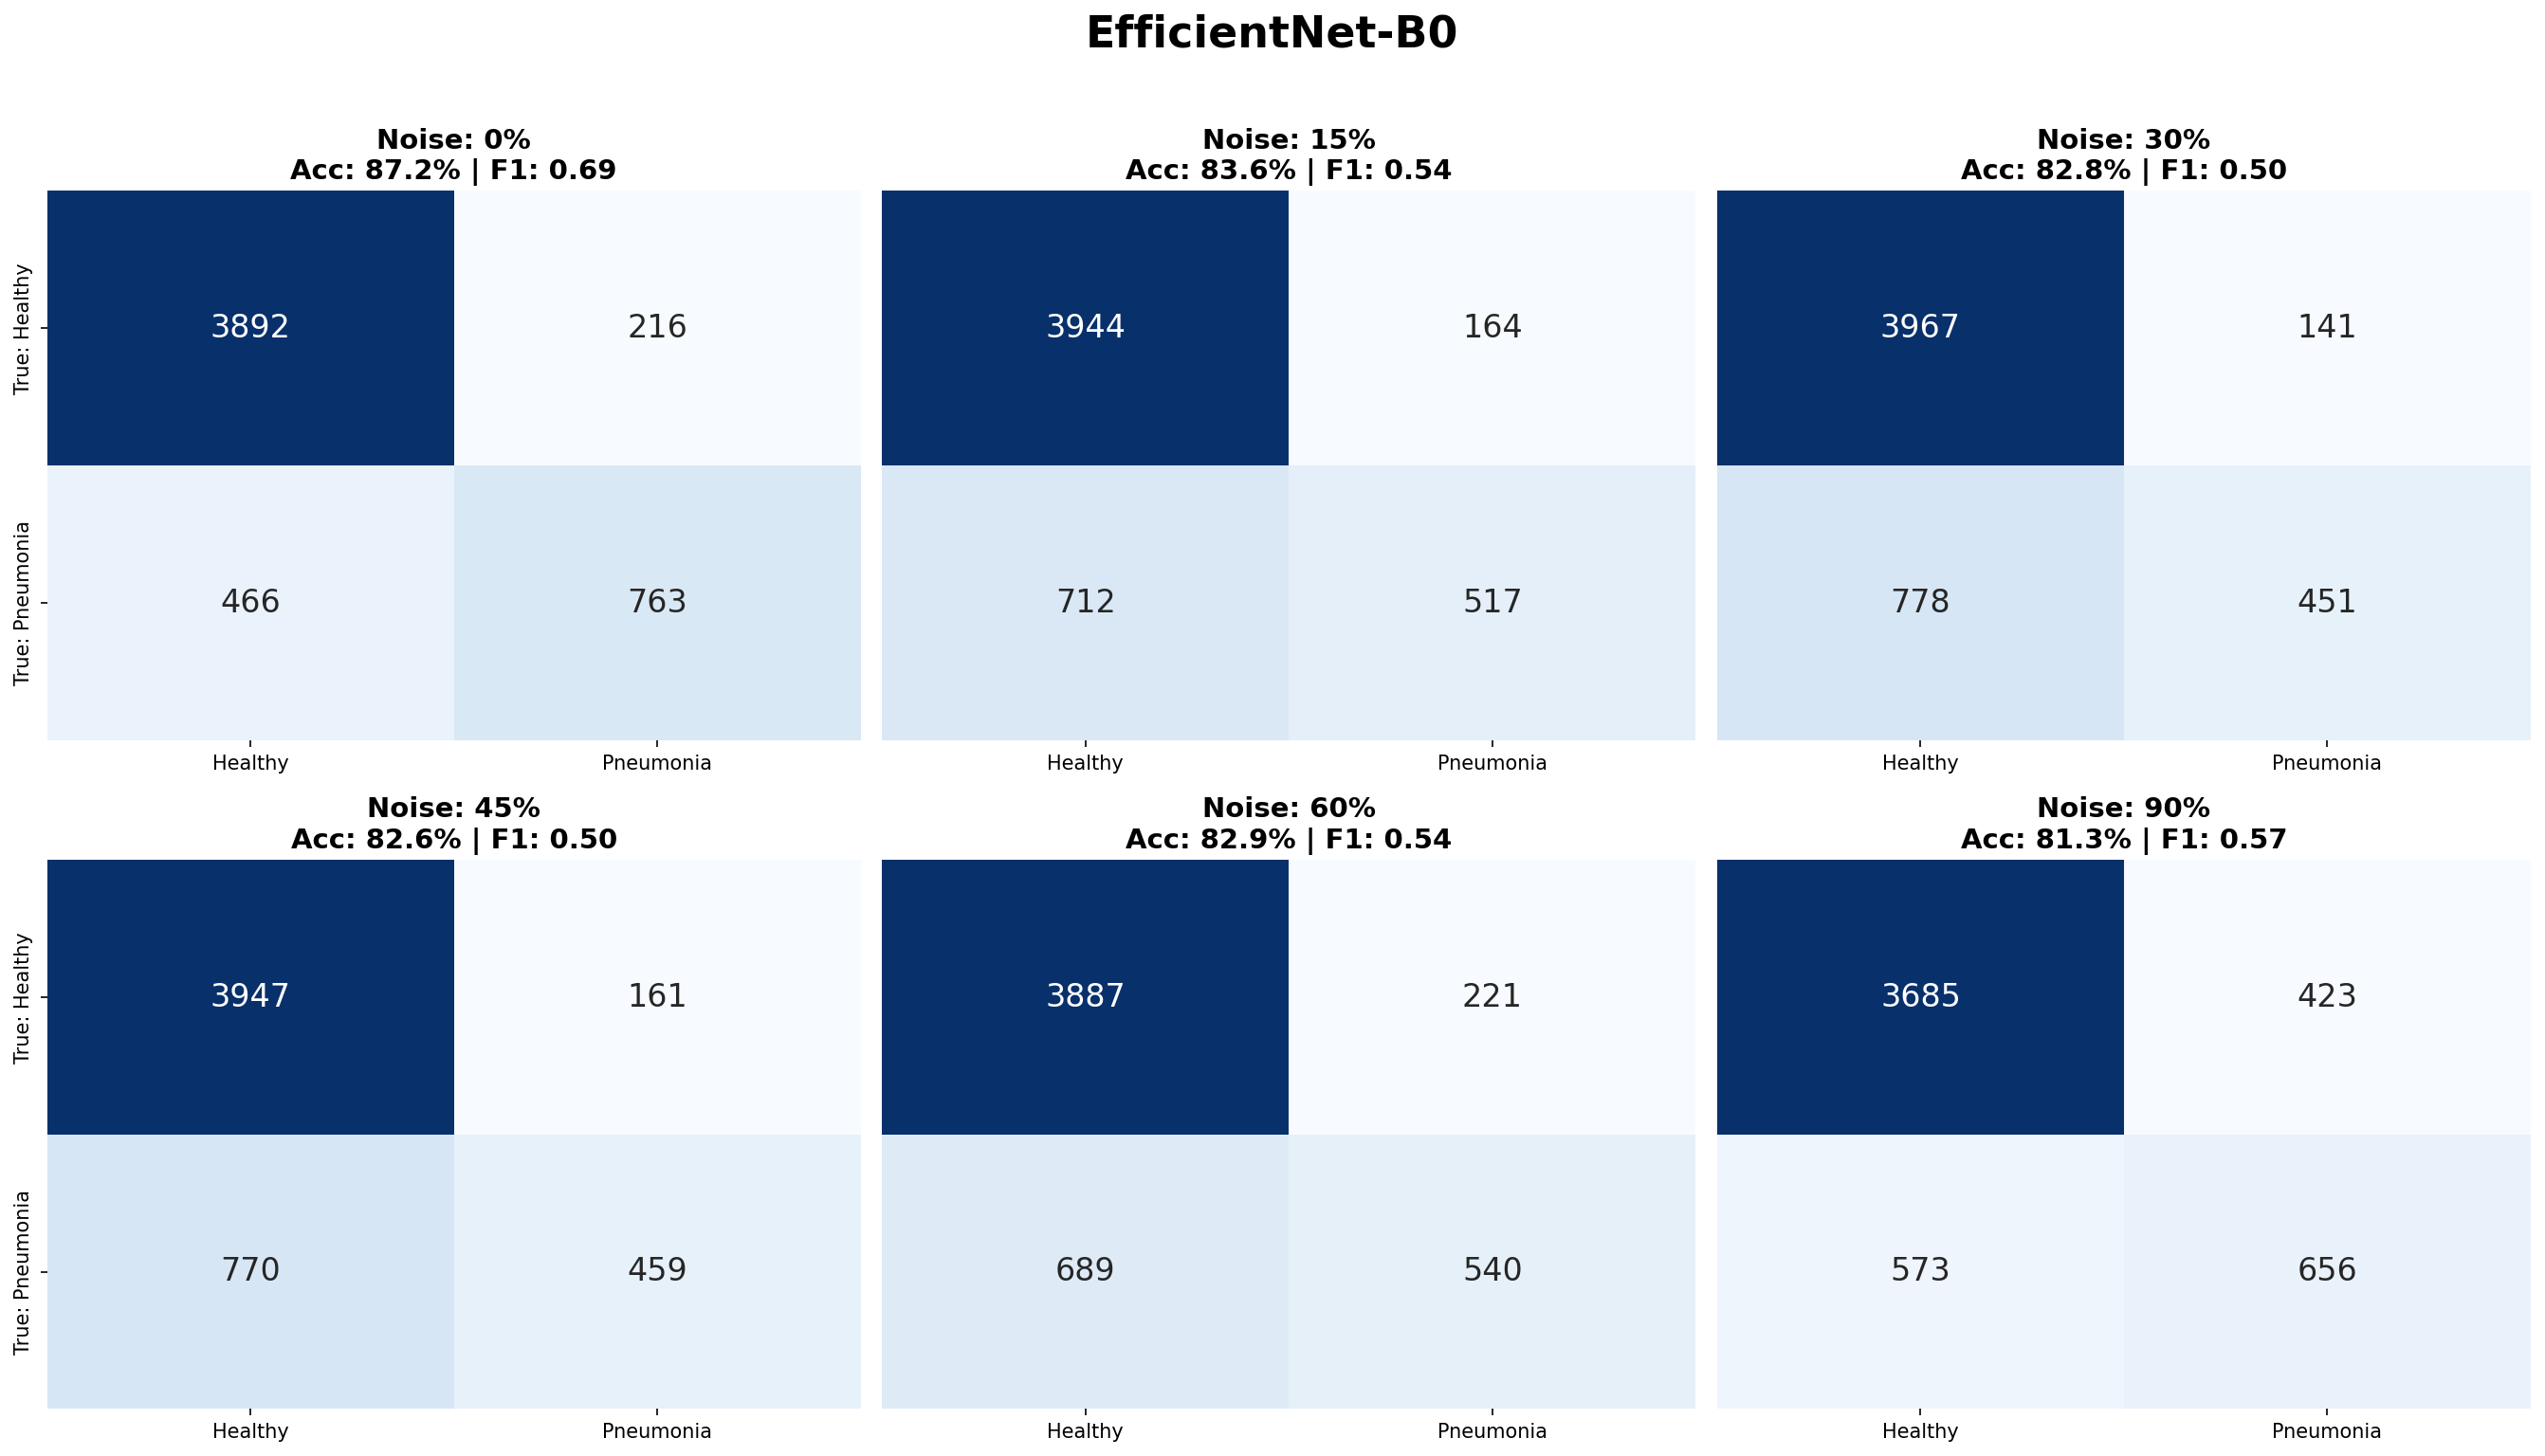
\includegraphics[width=0.85\linewidth]{figs/conf_matr_noise/EfficientNet-B0_CM.png}
		\caption{EfficientNet-B0}
		\label{fig:sub_efficientnet}
	\end{subfigure}
	\vspace{1em}
	
	\begin{subfigure}{\linewidth}
		\centering
		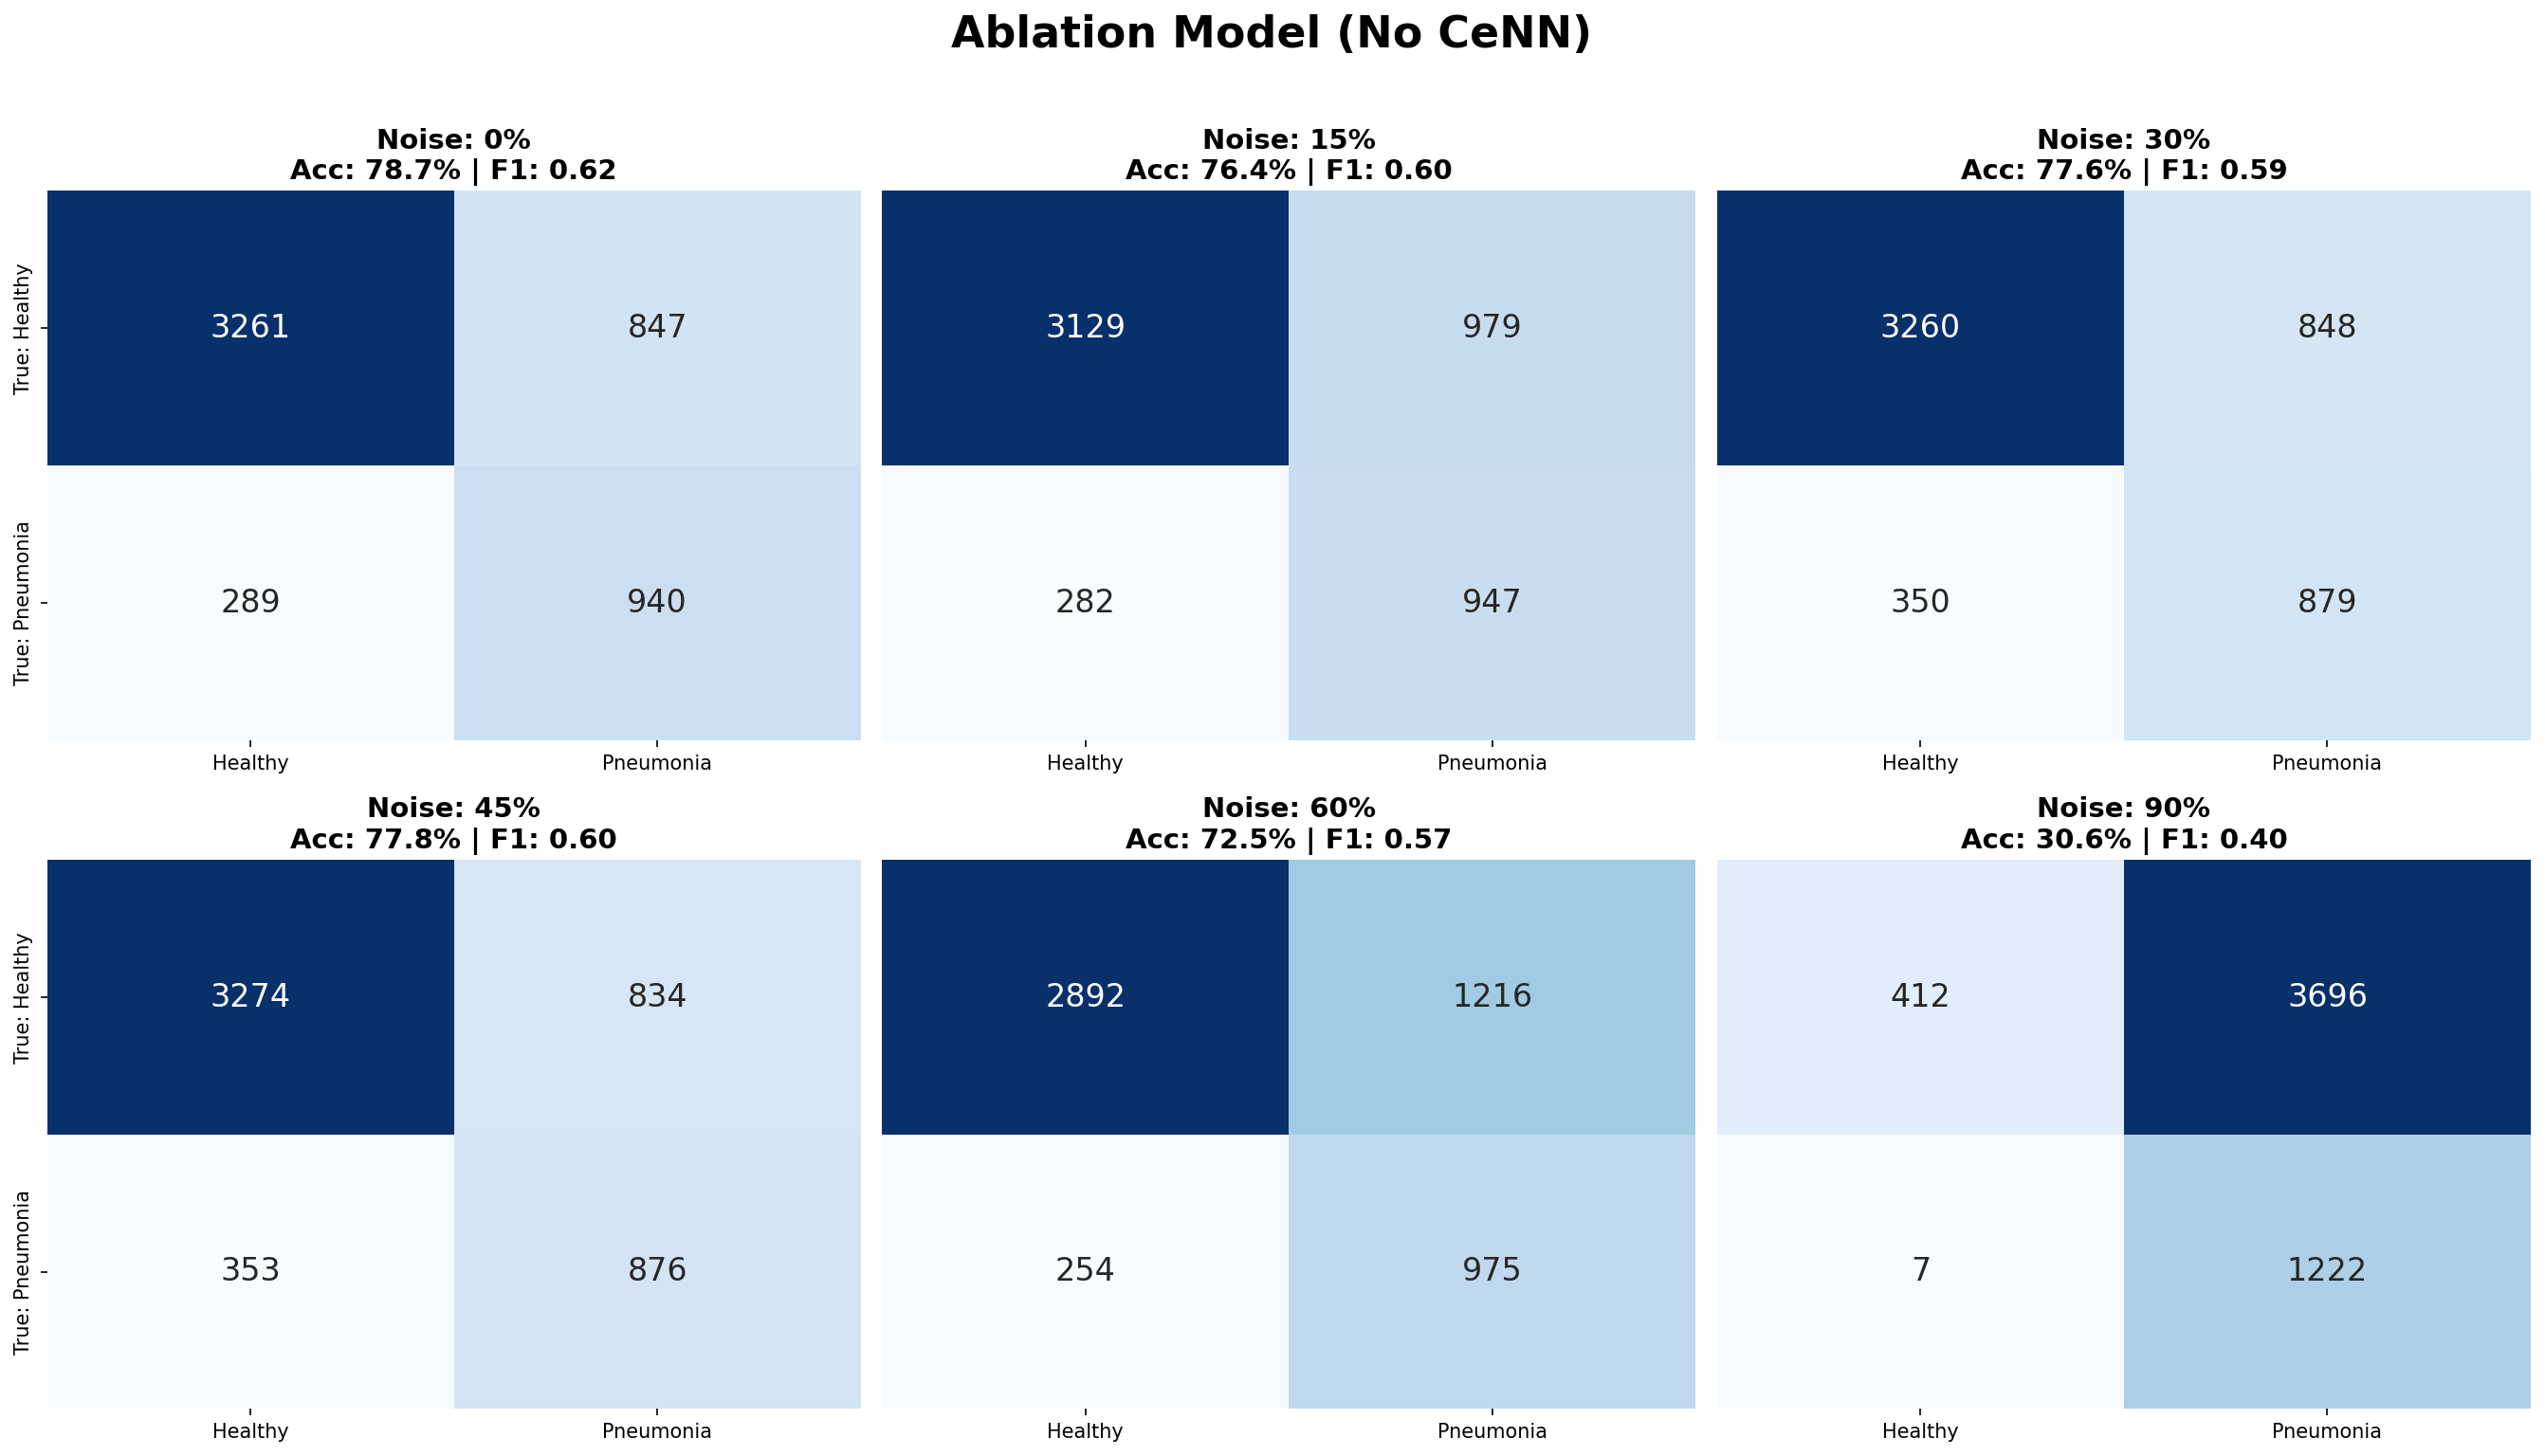
\includegraphics[width=0.85\linewidth]{figs/conf_matr_noise/Ablation_Model_(No_CeNN)_CM.png}
		\caption{Ablation Baseline (DenseNet-121 Without CeNN)}
		\label{fig:sub_nocenn}
	\end{subfigure}
	
	\caption{Detailed Confusion Matrices across different architectures (Part 2).}
	\label{fig:noise_comparison_p2}
\end{figure*}

% --- BLOCCO 3: Quinta immagine ---
\begin{figure*}[htbp]
	\ContinuedFloat 
	\centering
	\begin{subfigure}{\linewidth}
		\centering
		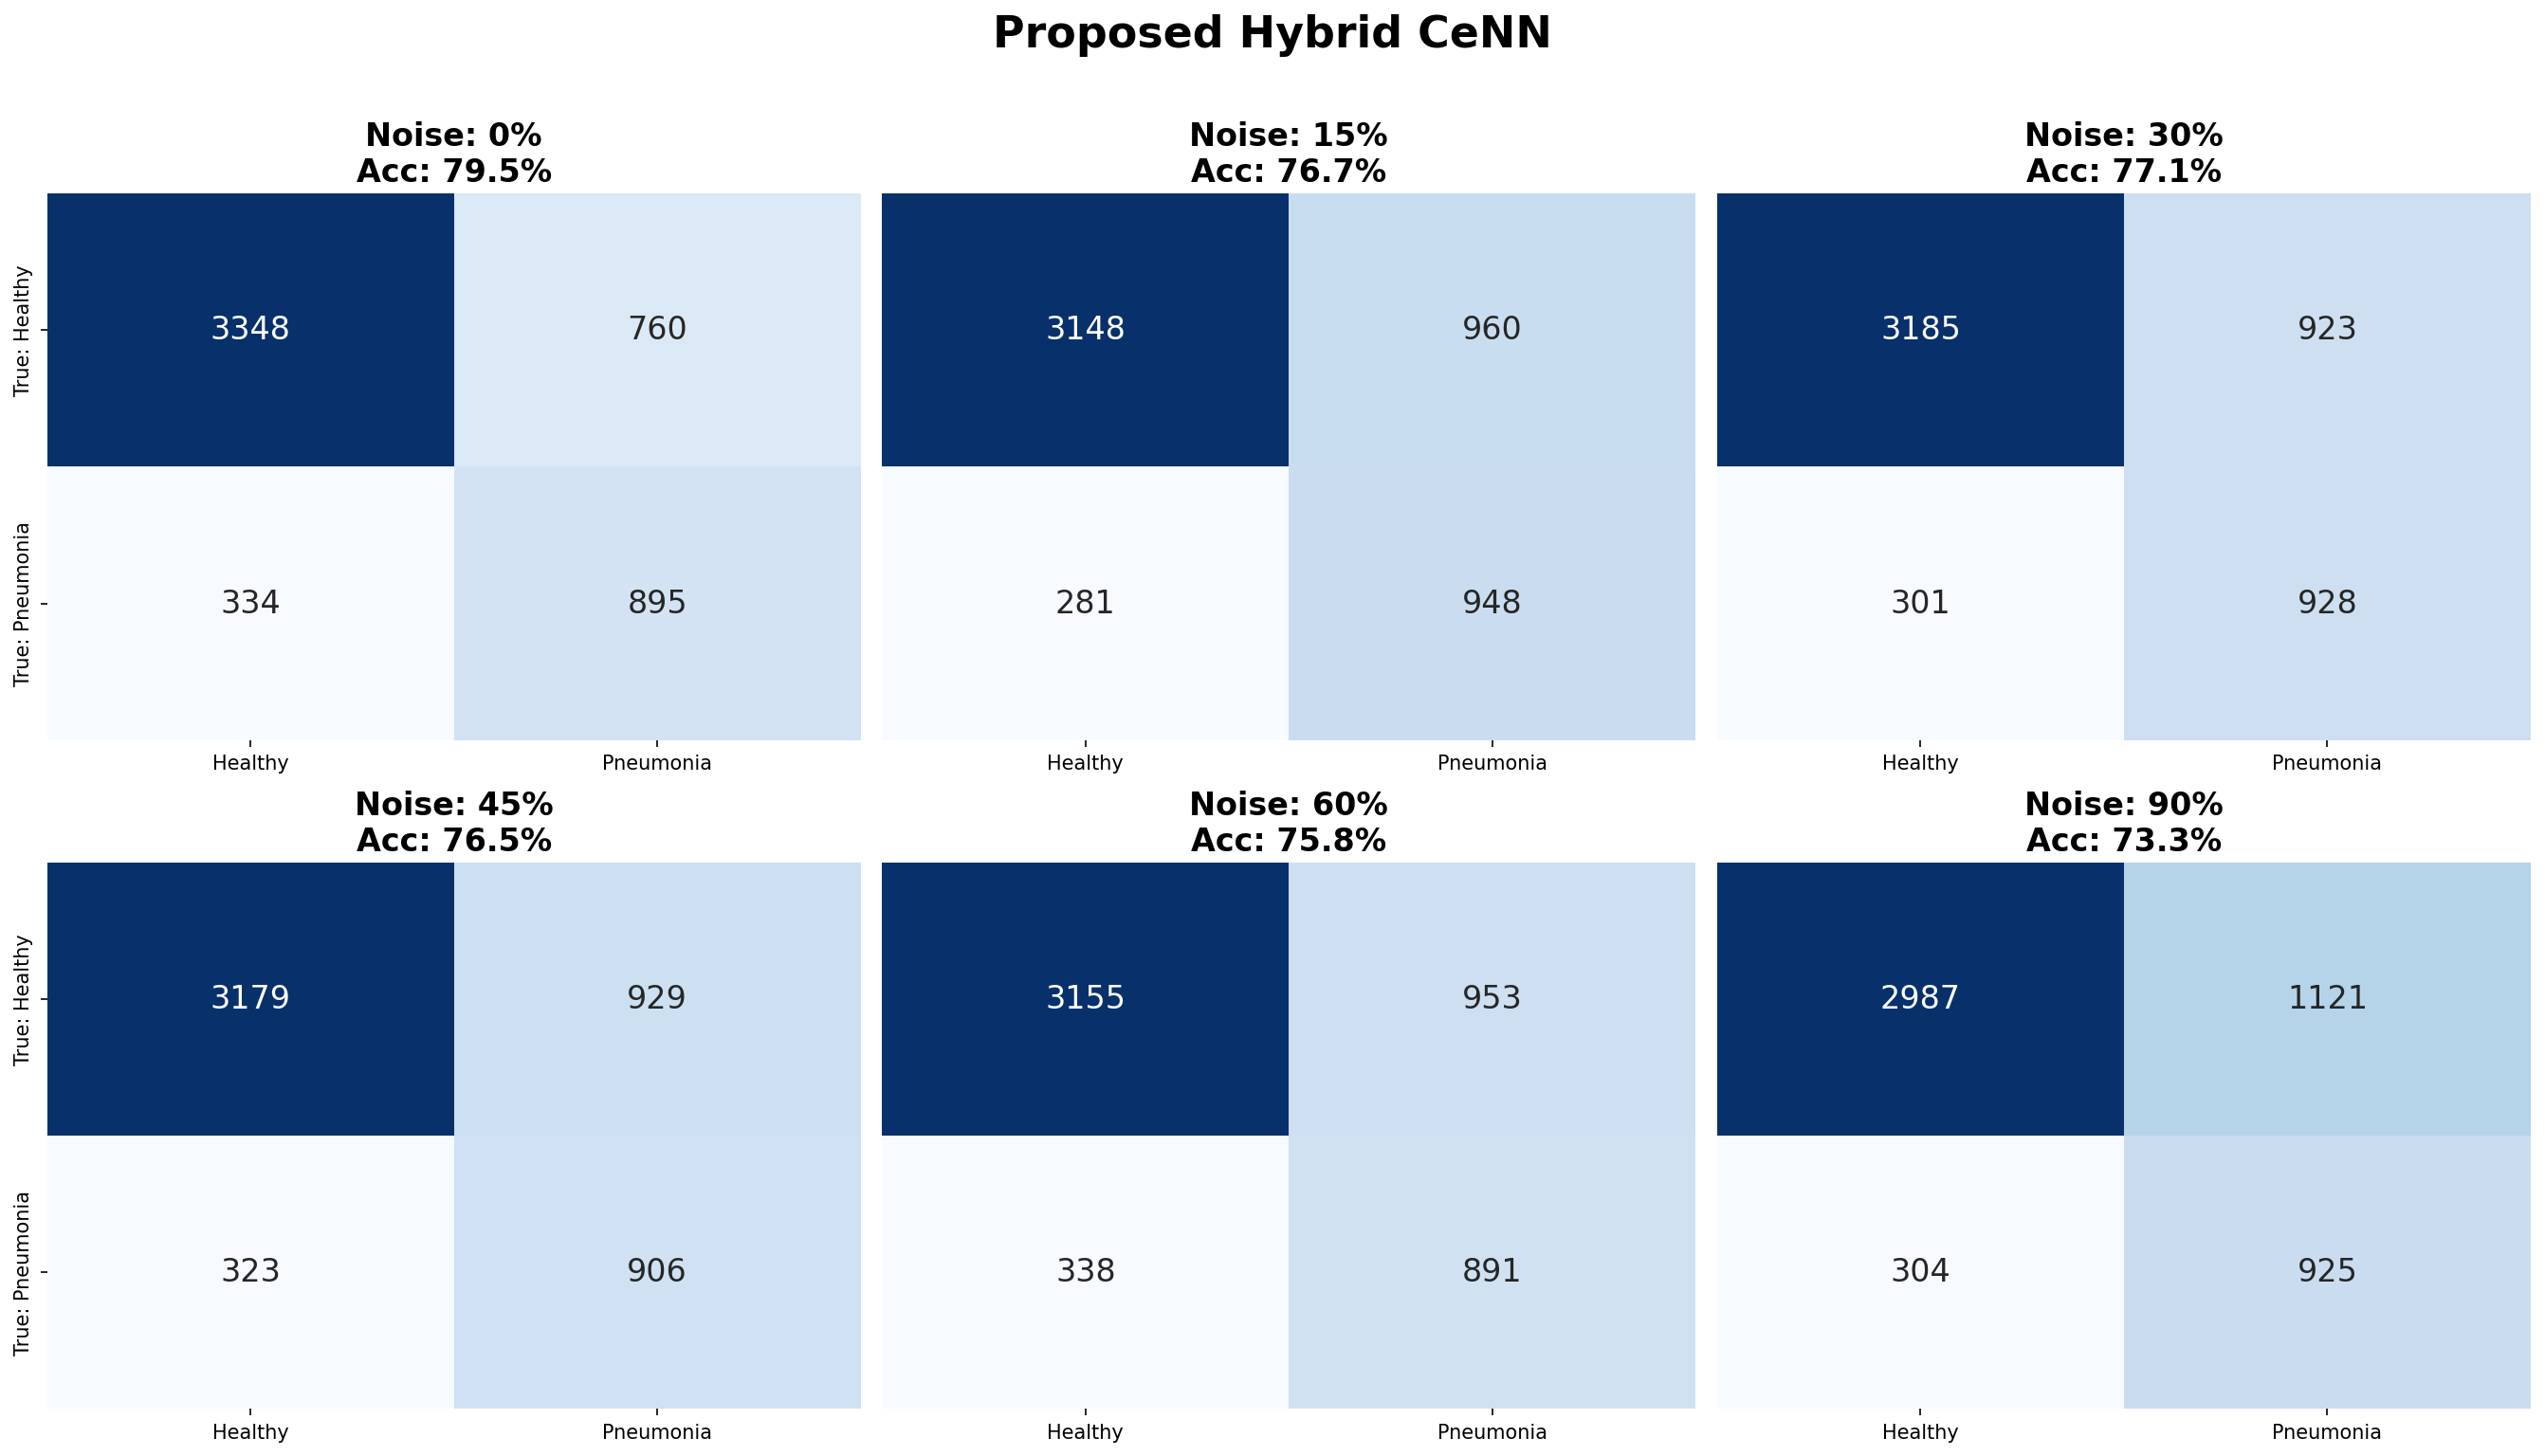
\includegraphics[width=0.85\linewidth]{figs/conf_matr_noise/Proposed_Hybrid_CeNN_CM.png}
		\caption{Proposed Hybrid CeNN}
		\label{fig:sub_nostro}
	\end{subfigure}
	
	\caption{Detailed Confusion Matrices across different architectures (Part 3)}
	\label{fig:noise_comparison_p3}
\end{figure*}
	% \section{Bibliography styles}
	
	% There are various bibliography styles available. You can select the
	% style of your choice in the preamble of this document. These styles are
	% Elsevier styles based on standard styles like Harvard and Vancouver.
	% Please use Bib\TeX\ to generate your bibliography and include DOIs
	% whenever available.
	
	% Here are two sample references: 
	% \cite{cbam}
	% \cite{Fortunato2010,NewmanGirvan2004}
	% \cite{Fortunato2010,Vehlowetal2013}
	
	
	
	% \section{Floats}
	% {Figures} may be included using the command,\linebreak 
	% \verb+\includegraphics+ in
	% combination with or without its several options to further control
	% graphic. \verb+\includegraphics+ is provided by {graphic[s,x].sty}
	% which is part of any standard \LaTeX{} distribution.
	% {graphicx.sty} is loaded by default. \LaTeX{} accepts figures in
	% the postscript format while pdf\LaTeX{} accepts {*.pdf},
	% {*.mps} (metapost), {*.png} and {*.png} formats. 
	% pdf\LaTeX{} does not accept graphic files in the postscript format. 
	
	
	
	% The \verb+table+ environment is handy for marking up tabular
	% material. If users want to use {multirow.sty},
	% {array.sty}, etc., to fine control/enhance the tables, they
	% are welcome to load any package of their choice and
	% {cas-dc.cls} will work in combination with all loaded
	% packages.
	
	% \begin{table}[width=.9\linewidth,cols=4,pos=h]
		% \caption{This is a test caption. This is a test caption. This is a test
			% caption. This is a test caption. Use \{table*\} instead of \{table\} if you
			% want a two column spanned table.}\label{tbl1}
		% \begin{tabular*}{\tblwidth}{@{} LLLL@{} }
			% \toprule
			% Col 1 & Col 2 & Col 3 & Col4\\
			% \midrule
			% 12345 & 12345 & 123 & 12345 \\
			% 12345 & 12345 & 123 & 12345 \\
			% 12345 & 12345 & 123 & 12345 \\
			% 12345 & 12345 & 123 & 12345 \\
			% 12345 & 12345 & 123 & 12345 \\
			% \bottomrule
			% \end{tabular*}
		% \end{table}
	
	% \section[Theorem and ...]{Theorem and theorem like environments}
	
	% {cas-dc.cls} provides a few shortcuts to format theorems and
	% theorem-like environments with ease. In all commands the options that
	% are used with the \verb+\newtheorem+ command will work exactly in the same
	% manner. {cas-dc.cls} provides three commands to format theorem or
	% theorem-like environments: 
	
	% \begin{verbatim}
		%  \newtheorem{theorem}{Theorem}
		%  \newtheorem{lemma}[theorem]{Lemma}
		%  \newdefinition{rmk}{Remark}
		%  \newproof{pf}{Proof}
		%  \newproof{pot}{Proof of Theorem \ref{thm2}}
		% \end{verbatim}
	
	
	% The \verb+\newtheorem+ command formats a
	% theorem in \LaTeX's default style with italicized font, bold font
	% for theorem heading and theorem number at the right hand side of the
	% theorem heading.  It also optionally accepts an argument which
	% will be printed as an extra heading in parentheses. 
	
	% \begin{verbatim}
		%   \begin{theorem} 
			%    For system (8), consensus can be achieved with 
			%    $\|T_{\omega z}$ ...
			%      \begin{eqnarray}\label{10}
				%      ....
				%      \end{eqnarray}
			%   \end{theorem}
		% \end{verbatim}  
	
	
	% \newtheorem{theorem}{Theorem}
	
	% \begin{theorem}
		% For system (8), consensus can be achieved with 
		% $\|T_{\omega z}$ ...
		% \begin{eqnarray}\label{10}
			% ....
			% \end{eqnarray}
		% \end{theorem}
	
	% The \verb+\newdefinition+ command is the same in
	% all respects as its \verb+\newtheorem+ counterpart except that
	% the font shape is roman instead of italic.  Both
	% \verb+\newdefinition+ and \verb+\newtheorem+ commands
	% automatically define counters for the environments defined.
	
	% The \verb+\newproof+ command defines proof environments with
	% upright font shape.  No counters are defined. 
	
	% \begin{figure*}
		% 	\centering
		% 	\includegraphics[width=.9\textwidth]{figs/cas-munnar-2024.png}
		% 	\caption{The beauty of Munnar, Kerala. (See also Table \protect\ref{tbl1}).}
		% 	\label{FIG:2}
		% \end{figure*}
	
	
	% \section[Enumerated ...]{Enumerated and Itemized Lists}
	% {cas-dc.cls} provides an extended list processing macros
	% which makes the usage a bit more user friendly than the default
	% \LaTeX{} list macros.   With an optional argument to the
	% \verb+\begin{enumerate}+ command, you can change the list counter
		% type and its attributes.
		
		% \begin{verbatim}
			%  \begin{enumerate}[1.]
				%  \item The enumerate environment starts with an optional
				%    argument `1.', so that the item counter will be suffixed
				%    by a period.
				%  \item You can use `a)' for alphabetical counter and '(i)' 
				%   for roman counter.
				%   \begin{enumerate}[a)]
					%     \item Another level of list with alphabetical counter.
					%     \item One more item before we start another.
					%     \item One more item before we start another.
					%     \item One more item before we start another.
					%     \item One more item before we start another.
					% \end{verbatim}
				
				% Further, the enhanced list environment allows one to prefix a
				% string like `step' to all the item numbers.  
				
				% \begin{verbatim}
					%  \begin{enumerate}[Step 1.]
						%   \item This is the first step of the example list.
						%   \item Obviously this is the second step.
						%   \item The final step to wind up this example.
						%  \end{enumerate}
					% \end{verbatim}
				
				% \section{Cross-references}
				% In electronic publications, articles may be internally
				% hyperlinked. Hyperlinks are generated from proper
				% cross-references in the article.  For example, the words
				% \textcolor{black!80}{Fig.~1} will never be more than simple text,
				% whereas the proper cross-reference \verb+\ref{tiger}+ may be
				% turned into a hyperlink to the figure itself:
				% \textcolor{blue}{Fig.~1}.  In the same way,
				% the words \textcolor{blue}{Ref.~[1]} will fail to turn into a
				% hyperlink; the proper cross-reference is \verb+\cite{Knuth96}+.
				% Cross-referencing is possible in \LaTeX{} for sections,
				% subsections, formulae, figures, tables, and literature
				% references.
				
				% \section{Bibliography}
				
				% Two bibliographic style files (\verb+*.bst+) are provided ---
				% {model1-num-names.bst} and {model2-names.bst} --- the first one can be
				% used for the numbered scheme. This can also be used for the numbered
				% with new options of {natbib.sty}. The second one is for the author year
				% scheme. When  you use model2-names.bst, the citation commands will be
				% like \verb+\citep+,  \verb+\citet+, \verb+\citealt+ etc. However when
				% you use model1-num-names.bst, you may use only \verb+\cite+ command.
				
				% \verb+thebibliography+ environment.  Each reference is a\linebreak
				% \verb+\bibitem+ and each \verb+\bibitem+ is identified by a label,
				% by which it can be cited in the text:
				
				% \noindent In connection with cross-referencing and
				% possible future hyperlinking it is not a good idea to collect
				% more that one literature item in one \verb+\bibitem+.  The
				% so-called Harvard or author-year style of referencing is enabled
				% by the \LaTeX{} package {natbib}. With this package the
				% literature can be cited as follows:
				
				% \begin{enumerate}[\textbullet]
					% \item Parenthetical: \verb+\citep{WB96}+ produces (Wettig \& Brown, 1996).
					% \item Textual: \verb+\citet{ESG96}+ produces Elson et al. (1996).
					% \item An affix and part of a reference:\break
					% \verb+\citep[e.g.][Ch. 2]{Gea97}+ produces (e.g. Governato et
					% al., 1997, Ch. 2).
					% \end{enumerate}
				
				% In the numbered scheme of citation, \verb+\cite{<label>}+ is used,
				% since \verb+\citep+ or \verb+\citet+ has no relevance in the numbered
				% scheme.  {natbib} package is loaded by {cas-dc} with
				% \verb+numbers+ as default option.  You can change this to author-year
				% or harvard scheme by adding option \verb+authoryear+ in the class
				% loading command.  If you want to use more options of the {natbib}
				% package, you can do so with the \verb+\biboptions+ command.  For
				% details of various options of the {natbib} package, please take a
				% look at the {natbib} documentation, which is part of any standard
				% \LaTeX{} installation.
				
				% \appendix
				% \section{My Appendix}
				% Appendix sections are coded under \verb+\appendix+.
				
				% \verb+\printcredits+ command is used after appendix sections to list 
				% author credit taxonomy contribution roles tagged using \verb+\credit+ 
				% in frontmatter.
				
				% \printcredits
				
				% %% Loading bibliography style file
				% %\bibliographystyle{model1-num-names}
				% \bibliographystyle{cas-model2-names}
				
				% % Loading bibliography database
				% \bibliography{cas-refs}
				
				
				% %\vskip3pt
				
				% \bio{}
				% Author biography without author photo.
				% Author biography. Author biography. Author biography.
				% Author biography. Author biography. Author biography.
				% Author biography. Author biography. Author biography.
				% Author biography. Author biography. Author biography.
				% Author biography. Author biography. Author biography.
				% Author biography. Author biography. Author biography.
				% Author biography. Author biography. Author biography.
				% Author biography. Author biography. Author biography.
				% Author biography. Author biography. Author biography.
				% \endbio
				
				% \bio{figs/cas-pic1}
				% Author biography with author photo.
				% Author biography. Author biography. Author biography.
				% Author biography. Author biography. Author biography.
				% Author biography. Author biography. Author biography.
				% Author biography. Author biography. Author biography.
				% Author biography. Author biography. Author biography.
				% Author biography. Author biography. Author biography.
				% Author biography. Author biography. Author biography.
				% Author biography. Author biography. Author biography.
				% Author biography. Author biography. Author biography.
				% \endbio
				
				% \bio{figs/cas-pic1}
				% Author biography with author photo.
				% Author biography. Author biography. Author biography.
				% Author biography. Author biography. Author biography.
				% Author biography. Author biography. Author biography.
				% Author biography. Author biography. Author biography.
				% \endbio
				
			\end{document}
			
